\documentclass[11pt]{article}

\usepackage{amsmath}
\usepackage[french, onelanguage]{algorithm2e}
\usepackage[french]{babel}
\usepackage{geometry}
\usepackage{glossaries}
\usepackage{graphicx}
\usepackage[hidelinks]{hyperref}
\usepackage[utf8]{inputenc}
\usepackage{listings}
\usepackage{lstautogobble}
\usepackage{tabularx}
\usepackage{tikz}
\usepackage{tocloft}
\usepackage{verbatim}
\usepackage{xcolor}

\makeglossaries

\newacronym{ansi}{ANSI}{American National Standard Institute}
\newacronym{ram}{RAM}{Random Access Memory}

\usetikzlibrary{calc, shapes.multipart, chains, arrows}

\geometry{
  a4paper,
  total={170mm,257mm},
  left=20mm,
  top=20mm,
}

\definecolor{RoyalBlue}{cmyk}{1, 0.50, 0, 0}

\lstset{language=C,
  keywordstyle=\color{RoyalBlue},
  basicstyle=\scriptsize\ttfamily,
  commentstyle=\ttfamily\itshape\color{darkgray},
  stringstyle=\ttfamily,
  breaklines=true,
  keepspaces=true,
  numbers=left,
  numbersep=5pt,
  showspaces=false,
  showstringspaces=false,
  showtabs=false,
  tabsize=4,
  autogobble=true
}

\title{Documentation Mini Projet Langage C}
\author{Caculli Giorgio LA196672, Tyranowski Jedrzej LA196937\\Haute École de Louvain en Hainaut (HELHa)}
\date{\today}

\begin{document}

\maketitle
\begin{abstract}
  Documentation pour le projet de Langage procédural sur les listes chaînées. Projet basé sur le concept
  d'un centre de formations.
\end{abstract}
%\small
\textbf{\textit{Mots-clés}} : liste, chaînée, c, noeud, centre, formation, tête

\newpage
\tableofcontents

\newpage
\section{Introduction}

\subsection{Le langage C}
La langage de programmation utilisé lors du développement et la mise en \oe{}uvre du programme est le
\texttt{ANSI-C}. Les différentes versions du langage disponibles lors du développement de ce programme sont:
\begin{itemize}
\item \textbf{ANSI-C} : La première vérsion standardisée par le \textbf{\acrlong{ansi}},
  abrégé en \textbf{\acrshort{ansi}} dans ce document, du langage \texttt{C} publiée en 1990.
\item \textbf{C-99} : Révision de la version \acrshort{ansi} pour permettre aux développeurs d'utiliser les
  commentaires \texttt{//}, les booléans grâce à la librairie \texttt{<stdbool.h>}, la déclaration des int
  directement dans la boucle \texttt{for}, et d'autres modérnisations de la syntaxe.
\item \textbf{C-11} : Mise à jour du langage \texttt{C} pour permettre le support des \texttt{thread} afin de pouvoir faire du multi-threading.
\item \textbf{C-17} : Révision de la version \textbf{C-11} qui n'ajoute aucune nouvelle fonctionnalité, mais
  corriges beaucoup bugs présents dans la version 11.
\end{itemize}
Dans les différentes applications que l'on a fait dans le cours de Langage procédural, la plupart des
interactions que l'on a eu avec le langage \texttt{C}, notammente le fait de devoir déclarer un \texttt{int}
avant une boucle \texttt{for}, ressemblaient fortement à l'\acrshort{ansi}-\texttt{C}. C'est pourquoi nous
avons choisi d'utiliser cette vérsion là.

\subsection{Fonctions générales utilisées}
Différentes fonctions ont été utilisée lors du développement de ce programme.\\
Voici une liste des fonctions clés utilisées:
\begin{itemize}
  
\item \texttt{fopen()} : Fonction qui sert à ouvrir un flux, la plupart du temps un fichier.\\
  Exemple :
  \begin{lstlisting}
    /* Admettons que le fichier donnees.dat existe */
    #include <stdio.h>
    int main() {
      FILE *fichier_in = fopen( "donnees.dat", "r" );
      /* On ouvre le fichier donnees.dat en lecture */
      FILE *fichier_out = fopen( "resultats.txt", "w" );
      /* Si le fichier resultats.txt n'existe pas on le cree, s'il existe toute information presente est ecrasee, puis on y accede en ecrite */
      return 0;
    }
  \end{lstlisting}

\item \texttt{fclose()} : Fonction qui sert à fermer tout flux ouvert.\\
  Exemple :
  \begin{lstlisting}
    /* Admettons que le fichier donnees.dat existe */
    #include <stdio.h>
    int main() {
      FILE *fichier_in = fopen( "donnees.dat", "r" );
      /* On ouvre le fichier donnees.dat en lecture */
      FILE *fichier_out = fopen( "resultats.txt", "w" );
      /* Si le fichier resultats.txt n'existe pas on le cree, s'il existe toute information presente est ecrasee, puis on y accede en ecrite */
      fclose( fichier_out );
      fclose( fichier_in );
      /* On ferme les fichiers lorsqu'on doit plus travailler avec eux */
      return 0;
    }
  \end{lstlisting}

  
\item \texttt{printf()} : Fonction qui sert à afficher une châine de caractères dans la console.\\
  Exemple:
  \begin{lstlisting}
    #include <stdio.h>
    int main() {
      printf( "Hello World!\n" ); /* Affiche "Hello World!" dans la console */
      return 0;
    }
  \end{lstlisting}
  
\item \texttt{fprintf()} : Fonction qui sert à écrire une chaîne de caractères vers un flux spécifique.\\
  Exemple:
  \begin{lstlisting}
    #include <stdio.h>
    int main() {
      File *ficher_sortie = fopen( "fichier_sortie.txt", "w" );
      /* On cree et on ouvre un fichier nomme fichier_sortie.txt en ecriture */
      fprintf( ficher_sortie, "Hello World!\n" );
      /* Ecrit "Hello World!" dans le ficher fichier_sortie.txt mais pas dans la console */
      fprintf( stdout, "Hello World!\n" );
      /* Affiche "Hello World!" dans la console mais pas dans le fichier de sortie */
      return 0;
    }
  \end{lstlisting}

\item \texttt{scanf()} : Fonction qui sert à extrapoler une entrée du clavier et stocker les informations extrapolées dans les paramètres déclarés dans la fonction.\\
  Exemple:
  \begin{lstlisting}
    #include <stdio.h>
    int main() {
      char prenom[50];
      int age;
      printf( "Comment t'appels-tu ? " );
      scanf( "%s", prenom ); /* Admettons que l'utilisateur insere "Jedrzej" */
      printf( "Quel age as-tu %s ? ", prenom );
      scanf( "%d", &age ); /* Admettons que l'utilisateur insere "21" */
      printf( "Salut %s, je vois que tu as %d ans!\n", prenom, age );
      /* Affiche "Salut Jedrzej, je vois que tu as 21 ans!" dans la console */
      return 0;
    }
  \end{lstlisting}
  
\item \texttt{fscanf()} : Fonction qui sert à extrapoler des entrées à partir d'un flux spécifique en respectant une structure précise, et stocker les informations extrapolées dans des paramètres déclarés dans la fonction.\\
  Exemple:
  \begin{lstlisting}
    /* Contenu dans ficher_entree.txt */
    /* Jedrzej 21 */
    #include <stdio.h>
    int main() {
      char prenom[50];
      int age;
      FILE *ficher_in = fopen( "fichier_entree.txt", "r" );
      /* On ouvre un fichier nomme fichier_entree.txt en lecture */
      fscanf( fichier_in, "%s %d\n", prenom, &age );
      /* On lit le contenu de fichier_entree.txt */
      printf( "Salut %s, je vois que tu as %d ans\n", prenom, age );
      /* Affiche "Salut Jedrzej, je vois que tu as 21 ans!" dans la console */
      return 0;
    }
  \end{lstlisting}
  
\item \texttt{fgets()} : Fonction qui a le même principe que fscanf, mais garde les espaces.\\
  Exemble :
  \begin{lstlisting}
    /* Contenu dans fichier_entree.txt */
    /* Caculli Giorgio 23 */
    #include <stdio.h>
    int main() {
      char nom_prenom[15];
      int age;
      FILE *fichier_in = fopen( "fichier_entree.txt", "r" );
      fgets( nom_prenom, 16, fichier_in );
      /* Lit les 15 caracteres depuis le fichier de donnees fichier_entree.txt */
      fscanf( fichier_in, "%d", &age );
      /* Lit l'age depuis le fichier de donnees fichier_entree.txt */
      printf( "%s %d\n", nom_prenom, age );
      /* Affiche "Caculli Giorgio 23" dans la console */
      return 0;
    }
  \end{lstlisting}
  
\item \texttt{strcpy()} : Fonction qui sert à copier une chaîne de caractères vers une autres chaîne de caractères.\\
  Exemple :
  \begin{lstlisting}
    #include <stdio.h>
    #include <string.h>
    int main() {
      char prenom[10];
      char source[10] = "Giorgio";
      strcpy( prenom, source );
      printf( "%s\n", prenom ); /* Affiche "Giorgio" dans la console */
      return 0;
    }
  \end{lstlisting}
  
\item \texttt{sizeof()} : Fonction qui renvoie la quantité de mémoire (en bytes) qu'une entité va occuper dans la \acrlong{ram}, ou mémoire vive en français, abrégé en \acrshort{ram} dans ce document.\\
  Exemple :
  \begin{lstlisting}
    #include <stdio.h>
    int main() {
      printf( "Taille de char: %lu\n", sizeof( char ) );
      /* Affiche 1 dans la console */
      printf( "Taille de int: %lu\n", sizeof( int ) );
      /* Affiche 4 dans la console */
      printf( "Taille de long: %lu\n", sizeof( long ) );
      /* Affiche 8 dans la console */
      printf( "Taille de int[4]: %lu\n", sizeof( int[4] ) );
      /* Affiche 16 dans la console, soit 4*4=16 */
      return 0;
    }
  \end{lstlisting}

\item \texttt{memcpy()} : Fonction qui copiés n octets depuis une zone mémoire vers une autre zone mémoire.\\
  Exemple :
  \begin{lstlisting}
    #include <stdio.h>
    #include <string.h>
    int main() {
      int src[] = {1, 2, 3};
      size_t n = sizeof(src) / sizeof(src[0])
      /* En sachant que la taille d'un int = 4 bytes, et qu'il y a 3 int dans src, on obtient 4 * 3 = 12 bytes utilises. On divise la taille totale du vecteur, soit 12, par la taille du premier element du vecteur, soit 4, donc 12 / 4 = 3 elements dans le vecteur */
      int dest[n]; /* On initialiser le vecteur dest avec la meme taille de src, ici 3 */
      memcpy( dest, src, sizeof(dest) ); /* On copie les informations de src vers dest */
      int i;
      for( i = 0; i < n; i++ ) {
        /* On parcourt tous les elements dans dest, du premier (indice 0) jusqu'au troisieme (indide 2) */
        printf( "%d ", dest[i] ); /* Affiche 1 2 3 dans la console */
      }
      return 0;
    }
  \end{lstlisting}
  
\item \texttt{getchar()} : Fonction qui sert à lire un caractère depuis un flux.\\
  Exemple:
  \begin{lstlisting}
    #include <stdio.h>
    int main() {
      char lettre;
      printf( "Inserez une lettre: " ); /* Admettons que l'utilisateur insere "a" */
      char c = getchar();
      printf( "Lettre inseree : %c\n", c );
      /* Affiche "a" dans la console */
    }
  \end{lstlisting}

\item \texttt{system()} : Fonction qui permet de lancer l'execution d'une commande sur le système d'exploitation hôte.\\
  Exemple:
  \begin{lstlisting}
    #include <stdlib.h>
    int main() {
      char *commande = "dir";
      system( commande );
      /* Execute la commande "dir", fonction qui sert a afficher ce qui est present dans le repertoire */
      return 0;
    }
  \end{lstlisting}

\item \texttt{calloc()} : Fonction qui permet de faire de l'allocation dynamique de mémoire.\\
  Exemple:
  \begin{lstlisting}
    #include <stdio.h>
    #include <stdlib.h>
    int main() {
      int *pointer;
      int i, n;
      printf( "Nombres d'elements a ajouter: " );
      scanf( "%d", &n ); /* Admettons que l'utilisateur insere 3 */
      pointer = ( int * ) calloc( n, sizeof( int ) );
      for( i = 0; i < n; i++ )
      {
        printf( "Entrez le numero N.%d ", i + 1 );
        scanf( "%d", &pointer[i] ); /* Admettons que l'utilisateur insere 1 2 et 3 */
      }
      for( i = 0; i < n; i++ )
      {
        printf( "%d ", pointer[i] );
        /* Affiche 1 2 3 dans la console */
      }
      return 0;
    }
  \end{lstlisting}
  
\end{itemize}

\subsubsection{Qu'est-ce l'allocation dynamique de mémoire?}
Une allocation dynamique de mémoire est le processus d'alluer de la mémoire lors de l'exécution d'un programme. Il existe quatre fonctions en \texttt{C} qui peuvent être utilisée pour allouer et libérer de la mémoire: \texttt{calloc()}, \texttt{free()}, \texttt{realloc()} et \texttt{malloc()}. Ces fonctions sont accéssible lors de l'introduction du header \texttt{<stdlib.h>} dans le code.

\subsubsection{Qu'est-ce \texttt{calloc()} ?}
\texttt{calloc()} est une fonction qui renvoie un pointeur vers un espace mémoire suffisamment libre pour stocker un tableau au nombre d'objets indéterminé et à la taille spécifiée. Si c'est pas le cas, la fonction renverra \texttt{NULL}. Le stockage est initialisé à zéro.

\subsubsection{Qu'est-ce \texttt{malloc()} ?}
\texttt{malloc()} est une fonction qui renvoie un pointeur vers un espace mémoire non initialisé. Si l'allocation n'est pas possible, la fonction renverra \texttt{NULL}. Si l'espace affecté par l'allocation est saturé, les résultats ne seront pas définis.

\subsubsection{Différences entre \texttt{calloc()} et \texttt{malloc()}}
\begin{center}
  \begin{tabularx}{\textwidth}{| >{\centering\arraybackslash}X | >{\centering\arraybackslash}X |}
    \hline
    \textbf{\texttt{malloc()}} & \textbf{\texttt{calloc()}} \\ 
    \hline
    \texttt{void * malloc( size\_t n );} & \texttt{void * calloc( size\_t n, size\_t size );} \\
    \hline
    \texttt{malloc()} prend un argument (le nombre d'octets)  & \texttt{calloc()} prend deux arguments (le nombre de blocs et la taille de chaque bloc)  \\
    \hline
    \texttt{malloc()} est plus rapide que \texttt{calloc()} & \texttt{calloc()} prends plus de temps que \texttt{malloc()} car la mémoire doit être initialisée à zéro \\
    \hline
  \end{tabularx}
\end{center}

\newpage
\section{Listes chaînées}
Voici une représentation d'une liste chaînée: 
\begin{tikzpicture}[list/.style={
      rectangle split,
      rectangle split parts=2,
      draw,
      rectangle split horizontal
    },
    >=stealth,
    start chain]

  \node[list,on chain] (A) {12};
  \node[list,on chain] (B) {99};
  \node[list,on chain] (C) {37};
  \node[on chain,draw,inner sep=6pt] (D) {};
  \draw (D.north east) -- (D.south west);
  \draw (D.north west) -- (D.south east);
  \draw[*->] let \p1 = (A.two), \p2 = (A.center) in (\x1,\y2) -- (B);
  \draw[*->] let \p1 = (B.two), \p2 = (B.center) in (\x1,\y2) -- (C);
  \draw[*->] let \p1 = (C.two), \p2 = (C.center) in (\x1,\y2) -- (D);
\end{tikzpicture}

\subsection{Qu'est-ce une liste chaînée?}
Une liste chaînée est une séquence de structures de données, qui sont liée par des n\oe{}uds.
Chaque n\oe{}ud contient une connexion vers un autre n\oe{}ud.\\
Il existe trois types de listes chaînées:
\begin{itemize}
\item La \textbf{liste chaînée linéaire} : Une liste chaînée que ne peut être parcourue dans une seule direction.
\item La \textbf{double liste chaînée} : Une liste chaînée qui peut être parcourue en deux directions: à partir de la tête ou à partir de la queue.
\item La \textbf{liste chaînée circulaire} : Une liste chaînée où le premier n\oe{}ud fait toujours référence au dernier n\oe{}ud.
\end{itemize}

Dans le cas de notre projet, on a travaillé avec la liste chaînée linéaire.\\
Voici à quoi ressemble une structure pour une liste chaînée linéaire en \texttt{C}:
\begin{lstlisting}
  typedef struct noeud
  {
    int donnee;         /* L'information que l'on souhaite stocker dans le noeud */
    struct noeud *suivant; /* Le lien vers le prochain noeud */
  } noeud;
  noeud *tete = NULL;   /* Le point de demarrage d'une liste chainee */
\end{lstlisting}

Contrairement à un vecteur, qui lui ressemblerait à ça:
\begin{lstlisting}
  int donnee[10];
\end{lstlisting}

Les deux vont très bien stocker des \texttt{int} que l'on a nommé \texttt{donnee}, cependant, un vecteur possède une taille fixe, il ne saura stocker que 10 éléments maximum dans notre cas. Tandis que dans le cas d'une liste chaînée, tant qu'il y a de l'espace en mémoire, il saura stocker un nombre indéfini de n\oe{}uds, et par conséquent, un nombre indéfini de \texttt{int donnee}.

\subsection{Création d'un nouveau n\oe{}ud}
Afin de pouvoir créer un n\oe{}ud que l'on stockera dans notre liste chaînée, il faudra d'abord lui alluoer une taille dans la mémoire. Toujours en se basant par le bout de code vu précédemment, et le bout de code vu dans le chapitre précédent sur l'allocation de mémoire, on obtiendrait le code suivant:
\begin{lstlisting}
  noeud *creer_noeud( int data )
  {
    noeud *temporaire = ( noeud * ) calloc( 1, sizeof( noeud ) );
    /* On cree un noeud temporaire ou l'on stockera les informations que l'on souhaite */
    temporaire->data = data; /* La donnee que l'on souhaite stocker */
    temporaire->suivant = NULL; /* Lien vers le prochain noeud s'il existe */
    return tmp; /* On retourne le noeud qui sera stocke dans la liste chainee */
  }
  noeud *treinte_sept = creer_noeud( 37 );
  free( treinte_sept );
\end{lstlisting}
Le résultat obtenu serait un n\oe{}ud du style:
\begin{tikzpicture}[list/.style={
      rectangle split,
      rectangle split parts=2,
      draw,
      rectangle split horizontal
    },
    >=stealth,
    start chain]
  \node[list,on chain] (C) {37};
\end{tikzpicture}

Le langage \texttt{C} ne fait pas de \texttt{Garbage Collection}, ce qui revient à dire que toute manipulation de mémoire doit être manipulée manuellement. Donc, lorsqu'on a besoin de libérer de la mémoire de données que l'on peut écraser, on utilise la fonction \texttt{free()}.\\
Dans ce cas-ci, le n\oe{}ud est créé mais il n'est pas encore stocké dans la liste chaînée.
On verra dans la section suivant comment on peut stocker ce nouveau noeud dans la liste chaînée.

\subsection{Insertion d'un n\oe{}ud dans une liste chaînée}
À l'état actuel des choses, on peut supposer que la liste chaînée soit vide: 
\begin{tikzpicture}[list/.style={
      rectangle split,
      rectangle split parts=2,
      draw,
      rectangle split horizontal
    },
    >=stealth,
    start chain]
  \node[on chain,draw,inner sep=6pt] (D) {};
  \draw (D.north east) -- (D.south west);
  \draw (D.north west) -- (D.south east);
\end{tikzpicture}\\
Une procédure d'ajout dans une liste chaînée pourrait être la suivante:
\begin{enumerate}
\item On initialise le noeud temporaire que l'on ajoutera à la base de données.
\item On associe \texttt{data} au pointeur \texttt{data} présent dans la structure \texttt{noeud}.
\item On initialise le prochain n\oe{}ud de la liste \texttt{*suivant} à NULL.
\item Si la tête \texttt{*tete} de la liste est \texttt{NULL}, alors la tête devient le nouveau n\oe{}ud. On arrête la fonction d'ajout là.
\item Sinon, on fait une copie de la tête dans le n\oe{}ud \texttt{*suivant} que l'on avait initialisé à \texttt{NULL}.
\item On déclare la tête comme étant le n\oe{}ud temporaire que l'on a initialisé.
\end{enumerate}
Dans une fonction, cette procédure ressemblerait à ça:
\begin{lstlisting}
  int ajouter_noeud( noeud *tete, int data )
  {
    noeud *temporaire = creer_noeud( data );
    /* On cree le noeud temporaire qui stocke la donnee */
    if( tete == NULL )
    {
      tete = temporaire;
      /* On le stocke directement temporaire a la place de tete si tete est NULL */
      return 1;
    }
    temporaire->suivant = tete;
    /* On fait une copie de tete (le noeud stocke precedemment) dans le suivant du noeud temporaire (au lieu de le laisser a NULL) */
    tete = temporaire;
    /* On fait devenir le noeud temporaire la nouvelle tete */
    return 1;
  }
  noeud *tete = NULL;
  ajouter_noeud( tete, 37 );
\end{lstlisting}
Si la fonction a réussi, la liste chaînée ressemblera à ça: 
\begin{tikzpicture}[list/.style={
      rectangle split,
      rectangle split parts=2,
      draw,
      rectangle split horizontal
    },
    >=stealth,
    start chain]
  \node[list,on chain] (C) {37};
  \node[on chain,draw,inner sep=6pt] (D) {};
  \draw (D.north east) -- (D.south west);
  \draw (D.north west) -- (D.south east);
  \draw[*->] let \p1 = (C.two), \p2 = (C.center) in (\x1,\y2) -- (D);
\end{tikzpicture}

Admettons que l'on souhaite ajouter une autre donnée à notre liste chaînée, on refait appel à la fonction:
\begin{lstlisting}[firstnumber=16]
  ajouter_noeud( tete, 99 );
\end{lstlisting}

Si la fonction a réussi, la liste chaînée ressemblera à ça:
\begin{tikzpicture}[list/.style={
      rectangle split,
      rectangle split parts=2,
      draw,
      rectangle split horizontal
    },
    >=stealth,
    start chain]
  \node[list,on chain] (B) {99};
  \node[list,on chain] (C) {37};
  \node[on chain,draw,inner sep=6pt] (D) {};
  \draw (D.north east) -- (D.south west);
  \draw (D.north west) -- (D.south east);
  \draw[*->] let \p1 = (B.two), \p2 = (B.center) in (\x1,\y2) -- (C);
  \draw[*->] let \p1 = (C.two), \p2 = (C.center) in (\x1,\y2) -- (D);
\end{tikzpicture}

\subsection{Suppression d'un n\oe{}ud d'une liste chaînée}

Pour que l'on puisse supprimer un n\oe{}ud, il faudra d'abord passer par différentes étapes de vérification:
\begin{enumerate}
\item On vérife que la tête de la liste \texttt{*tete} ne soit pas \texttt{NULL}, si oui, on arrête la fonction.
\item On vérifie si le premier élément de la liste correspond à la donnée \texttt{data} de la liste que l'on souhaite supprimer.
\item Si oui:
  \begin{enumerate}
  \item On crée un n\oe{}ud temporaire qui stockera la donnée suivante dans la liste.
  \item On libére l'espace mémoire occupé par head avec la fonction \texttt{free(tete)}.
  \item On attribue à \texttt{tete} le n\oe{}ud temporaire que l'on avait créé.
  \item On arrête la fonction.
  \end{enumerate}
\item Sinon, on parcourt l'entièreté de la liste jusqu'au moment où l'on trouve la formation qui a le même \texttt{donnee} que la \texttt{donnee} en paramètre.
\item Si on le trouve, on pivote l'élément qui suit vers l'élément que l'on vient de supprimer.
\item On arrête la fonction, si réussite, on obtient 1, si pas, on obtient 0.
\end{enumerate}

Cette procédure pourrait être écrite de la manière suivante:
\begin{lstlisting}
  int supprimer_noeud( noeud *tete, int data )
  {
    if( tete == NULL )
    {
      return 0;
    }
    noeud *temporaire = NULL;
    if( tete->data == data )
    {
      temporaire = tete->suivant;
      free( tete );
      tete = temporaire;
      return 1;
    }
    while( tete != NULL )
    {
      if( tete->suivant->data == data )
      {
        temporaire = tete->suivant;
        tete->suivant = tete->suivant->suivant;
        free( temporaire );
        return 1;
      }
      tete = tete->suivant;
    }
    return 0;
  }
  noeud *tete = NULL;
  ajouter_noeud( tete, 37 );
  ajouter_noeud( tete, 99 );
  ajouter_noeud( tete, 42 );
  ajouter_noeud( tete, 12 );
  ajouter_noeud( tete, 10 );
  supprimer_noeud( tete, 10 );
  supprimer_noeud( tete, 42 );
\end{lstlisting}

Analysons ce que le code fait:
\begin{enumerate}
  \setcounter{enumi}{27}
\item On crée la tête à NULL
\item On ajoute dans la liste chaînée la variable 37 qui sera stockée dans un n\oe{}ud.
\item On ajoute dans la liste chaînée la variable 99 qui sera stockée dans un n\oe{}ud.
\item On ajoute dans la liste chaînée la variable 42 qui sera stockée dans un n\oe{}ud.
\item On ajoute dans la liste chaînée la variable 12 qui sera stockée dans un n\oe{}ud.
\item On ajoute dans la liste chaînée la variable 10 qui sera stockée dans un n\oe{}ud.\\
  À l'état actuel des choses, la liste ressemble à ça:\\\\
  \begin{tikzpicture}[list/.style={
        rectangle split,
        rectangle split parts=2,
        draw,
        rectangle split horizontal
      },
      >=stealth,
      start chain]

    \node[list,on chain] (A) {10};
    \node[list,on chain] (B) {12};
    \node[list,on chain] (C) {42};
    \node[list,on chain] (D) {99};
    \node[list,on chain] (E) {37};
    \node[on chain,draw,inner sep=6pt] (F) {};
    \draw (F.north east) -- (F.south west);
    \draw (F.north west) -- (F.south east);
    \draw[*->] let \p1 = (A.two), \p2 = (A.center) in (\x1,\y2) -- (B);
    \draw[*->] let \p1 = (B.two), \p2 = (B.center) in (\x1,\y2) -- (C);
    \draw[*->] let \p1 = (C.two), \p2 = (C.center) in (\x1,\y2) -- (D);
    \draw[*->] let \p1 = (D.two), \p2 = (D.center) in (\x1,\y2) -- (E);
    \draw[*->] let \p1 = (E.two), \p2 = (E.center) in (\x1,\y2) -- (F);
  \end{tikzpicture}
\item On supprime le noeud avec la valeur 10.
\item On supprime le noeud avec la valeur 42.\\
  Au final la liste ressemblera à ça:\\\\
  \begin{tikzpicture}[list/.style={
        rectangle split,
        rectangle split parts=2,
        draw,
        rectangle split horizontal
      },
      >=stealth,
      start chain]

    \node[list,on chain] (A) {12};
    \node[list,on chain] (B) {99};
    \node[list,on chain] (C) {37};
    \node[on chain,draw,inner sep=6pt] (D) {};
    \draw (D.north east) -- (D.south west);
    \draw (D.north west) -- (D.south east);
    \draw[*->] let \p1 = (A.two), \p2 = (A.center) in (\x1,\y2) -- (B);
    \draw[*->] let \p1 = (B.two), \p2 = (B.center) in (\x1,\y2) -- (C);
    \draw[*->] let \p1 = (C.two), \p2 = (C.center) in (\x1,\y2) -- (D);
  \end{tikzpicture}
\end{enumerate}

Voici comment la suppression interagit avec la liste chaînée et le nombre 10:
\begin{enumerate}
\item Est-ce que le liste est vide? (\texttt{tete == NULL} ?)
  \begin{enumerate}
  \item Non car on a des noeuds dans notre liste, on continue dans la fonction.
  \end{enumerate}
\item Est-ce que la donnée \texttt{data} équivaut à la donnée \texttt{tete->donnee} ?
  \begin{enumerate}
  \item Oui car \texttt{tete->donnee = 10} et \texttt{data = 10}.
  \end{enumerate}
\item On fait un backup de \texttt{tete->suivant} dans un n\oe{}ud temporaire.
\item On libére le n\oe{}ud \texttt{tete}.
\item On attribue à \texttt{tete} le n\oe{}ud temporaire.\\
  A ce stade de la modification, la liste ressemble à ça:\\\\
  \begin{tikzpicture}[list/.style={
        rectangle split,
        rectangle split parts=2,
        draw,
        rectangle split horizontal
      },
      >=stealth,
      start chain]
    \node[list,on chain] (B) {12};
    \node[list,on chain] (C) {42};
    \node[list,on chain] (D) {99};
    \node[list,on chain] (E) {37};
    \node[on chain,draw,inner sep=6pt] (F) {};
    \draw (F.north east) -- (F.south west);
    \draw (F.north west) -- (F.south east);
    \draw[*->] let \p1 = (B.two), \p2 = (B.center) in (\x1,\y2) -- (C);
    \draw[*->] let \p1 = (C.two), \p2 = (C.center) in (\x1,\y2) -- (D);
    \draw[*->] let \p1 = (D.two), \p2 = (D.center) in (\x1,\y2) -- (E);
    \draw[*->] let \p1 = (E.two), \p2 = (E.center) in (\x1,\y2) -- (F);
  \end{tikzpicture}
\end{enumerate}

Voici comment la suppression interagit avec la liste chaînée et le nombre 42:
\begin{enumerate}
\item Est-ce que le liste est vide? (\texttt{tete == NULL} ?)
  \begin{enumerate}
  \item Non car on a des noeuds dans notre liste, on continue dans la fonction.
  \end{enumerate}
\item Est-ce que la donnée \texttt{data} équivaut à la donnée \texttt{tete->donnee} ?
  \begin{enumerate}
  \item Non car \texttt{tete->donnee = 12} et \texttt{data = 42}.
  \end{enumerate}
\item On commence à parcourir toute la liste tant que \texttt{tete != NULL}.
\item On vérifie si \texttt{tete->suivant->donnee == data}
  \begin{enumerate}
  \item Si c'est pas le cas, on continue à parcourir la liste.
  \end{enumerate}
\item Si c'est le cas, on fait un backup du suivant du suivant dans un n\oe{}ud temporaire.
\item On libère \texttt{tete->suivant}.
\item On attribue à \texttt{tete->suivant} le n\oe{}ud \texttt{tete->suivant->suivant} (on pivote la liste vers la gauche et on libère l'espace mémoire qui était occupée par le 42).\\
  A ce stade de la modification, la liste ressemble à ça:\\\\
  \begin{tikzpicture}[list/.style={
        rectangle split,
        rectangle split parts=2,
        draw,
        rectangle split horizontal
      },
      >=stealth,
      start chain]
    \node[list,on chain] (A) {12};
    \node[list,on chain] (B) {99};
    \node[list,on chain] (C) {37};
    \node[on chain,draw,inner sep=6pt] (D) {};
    \draw (D.north east) -- (D.south west);
    \draw (D.north west) -- (D.south east);
    \draw[*->] let \p1 = (A.two), \p2 = (A.center) in (\x1,\y2) -- (B);
    \draw[*->] let \p1 = (B.two), \p2 = (B.center) in (\x1,\y2) -- (C);
    \draw[*->] let \p1 = (C.two), \p2 = (C.center) in (\x1,\y2) -- (D);
  \end{tikzpicture}
\end{enumerate}

Si la fonction a réussi, on obtiendra 1 comme résultat, si non, on obtiendra 0.

\subsection{Affichage d'une liste chaînée}

Pour l'affichage d'une liste châinée, on parcourt l'entièreté de la liste chaînée \texttt{noeud}. Tant que la tête n'est pas \texttt{NULL}, on affichera les informations que l'on souhaite afficher de chaque n\oe{}ud présente dans la liste chaînée.\\
Généralement, le code en langage \texttt{C} ressemblerait à ça:
\begin{lstlisting}
  void afficher_liste( noeud *tete )
  {
    while( tete != NULL )
    {
      printf( "%d ", tete->donnee );
      /* Affiche 12 99 37 de maniere recursive */
      tete = tete->suivant;
    }
  }
  afficher_liste(tete);
\end{lstlisting}

Si on se base sur la liste chaînée:
\begin{tikzpicture}[list/.style={
      rectangle split,
      rectangle split parts=2,
      draw,
      rectangle split horizontal
    },
    >=stealth,
    start chain]
  \node[list,on chain] (A) {12};
  \node[list,on chain] (B) {99};
  \node[list,on chain] (C) {37};
  \node[on chain,draw,inner sep=6pt] (D) {};
  \draw (D.north east) -- (D.south west);
  \draw (D.north west) -- (D.south east);
  \draw[*->] let \p1 = (A.two), \p2 = (A.center) in (\x1,\y2) -- (B);
  \draw[*->] let \p1 = (B.two), \p2 = (B.center) in (\x1,\y2) -- (C);
  \draw[*->] let \p1 = (C.two), \p2 = (C.center) in (\x1,\y2) -- (D);
\end{tikzpicture}

Ce qui se passe dans le code est la manipulation suivante:
\begin{enumerate}
\item On vérifie si \texttt{tete} est différent de \texttt{NULL}.
\item Si c'est le cas, on affiche dans la console la valeur \texttt{tete->donnee}
\item On continue à parcourir la liste, donc \texttt{tete} devient \texttt{tete->suivant}
\item Même procédure tant que \texttt{tete != NULL}.
\end{enumerate}

Donc, l'affichage sera: 12 99 37 dans la console.

\newpage
\section{Énoncé}
Le centre de formations propose diverses formations dans différents domaines.\\\\
Chaque \textbf{formation} est caractérisée par:
\begin{itemize}
\item Un identifiant unique (un nombre entier)
\item Un nombre de prérequis (Un nombre entier de 0 à 10)
\item Les identifiants des formations qui seraient des prérequis (On suppose qu'une formation ne peut avoir que 10 prérequis maximum)
\item Le nombre de jours où la formations a lieu (un entier de 1 à 7)
\item Le jour précis (sous forme de int 1 - lundi, 2 - mardi, etc\ldots)
\item L'heure de début de la formation (en format 08.15)
\item La durée de la formation en heures (un nombre entier)
\item Un coût fixe (Un float positif, par exemple 175.55)
\item Un nom (40 caractères maximum)
\end{itemize}
Le nombre de formations est indéfini.\\\\
Un nombre indéfini de personnes peuvent participer à n'importe quelle formation, bien des formateurs que des étudiants.\\\\
Une \textbf{personne} est caractérisée par:
\begin{itemize}
\item Un identifiant unique (Un nombre entier)
\item Un nom de famille (25 caractères maximum)
\item Un prénom (25 caractères maximum)
\item S'il/elle est formateur ou pas (1 formateur, 0 étudiant)
\item Le nombre de formations auquel il/elle participe (On suppose que dans une année, une personne quelconque ne puisse participer qu'à 30 formations maximum)
\item Dans le cas d'un formateur, le nombre de jour où il/elle aurait des indisponibilités (de 1 à 7)
\item Suivi par le jours précis où il/elle aurait des indisponibilités (1 - lundi, 2 - mardi, etc\ldots) 
\item Dans le cas d'un étudiant, il se peut qu'il/elle ait droit à une remise. (1 - oui, 0 - non)
\item Si c'est le cas, le pourcentage de sa remise sera précisé (de 0 à 100)
\end{itemize}\leavevmode\newline
Points importants à maîtriser :
\begin{itemize}
\item Étant donné qu'il n'y a pas de nombre maximal de personnes qui peuvent être inscrits dans le centre de formations, et qu'il n'y a pas de nombre maximal de formations qu'un centre de formations puisse proposer, le stockage par vecteurs des diverses personnes et formations n'est pas permis. Dès lors il faut initialiser des listes chaînées qui stockeront les diverses informations.
\item Le logiciel doit pouvoir afficher la liste des personnes ainsi que la liste des formations, et à partir de ces données, générer un planning pour la semaine.
\item Il doit être également possible d'ajouter et de supprimer des nouvelles personne ou personnes dans leurs respectives bases de données.
\item La possibilité de pouvoir attribuer une personne à une formation et de pouvoir la retirer d'une formation doit être prise en compte.
\item Toutes les opérations doivent être dynamiques, donc, toute manipulation doit être possible à partir du moment où le programme est lancé jusqu'au moment où il est arrêté.
\end{itemize}

\newpage
\section{Programme}
Le programme saura faires les manipulations suivantes:
\begin{itemize}
\item Ajouter des nouvelles personnes ou formations dans leurs respectives bases de données
\item Supprimer des personnes ou des formations entièrement de leurs respectives bases de données
\item Supprimer une personne spécifique d'une formation spécifique
\item Afficher les informations stockées dans les respectives bases de données.
\item Afficher un planning de la semaine détaillé
\item Sauvegarder toute modification faite
\end{itemize}
En résultat, il est demandé d'obtenir le planning détaillé de la semaine dans un fichier \texttt{CaculliTyranowski.res}
\subsection{Mode d'emploi}
\subsubsection{Menu principale}
Tous les traitements se feront dans la console du logiciel en lisant l'entrée du clavier.
\begin{figure}[ht]
  \centering
  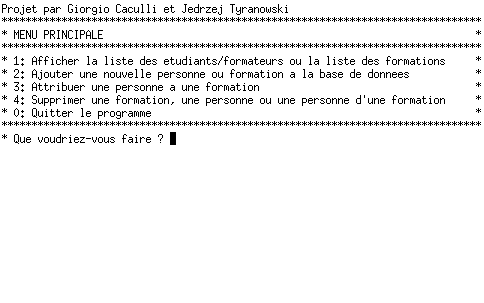
\includegraphics[trim=0 150 0 0, clip, scale=0.8]{images/01.png.png}
\end{figure}\\
Pour naviguer dans le menu, il faut frapper entre 0 et 4 sur le clavier et confirmer avec Enter.

\subsubsection{Menu affichage}
\begin{figure}[ht]
  \centering
  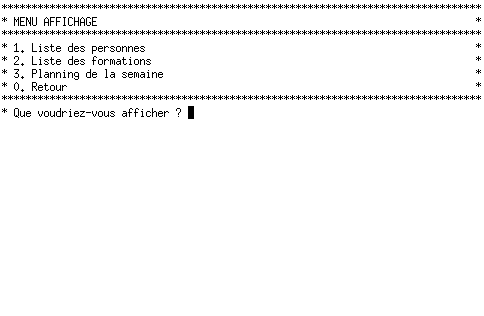
\includegraphics[trim=0 190 0 0, clip, scale=0.8]{images/02.png.png}
\end{figure}
Choisissez une option parmi 1, 2 et 3 et confirmez avec Enter pour continuer.

\newpage
\subsubsection{Liste des personnes}
\begin{figure}[ht]
  \centering
  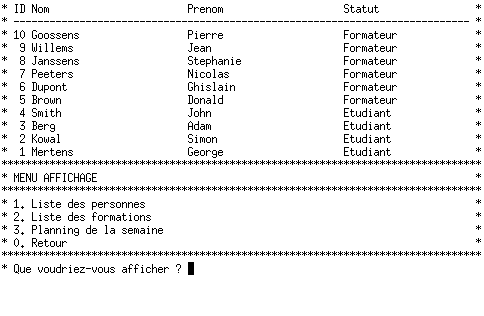
\includegraphics[trim=0 40 0 0, clip, scale=0.8]{images/03.png.png}
\end{figure}
Affiche l'ID, le nom de famille, le prénom et le statut (étudiant ou formateur) sous la forme d'une liste.

\subsubsection{Liste des formations}
\begin{figure}[ht]
  \centering
  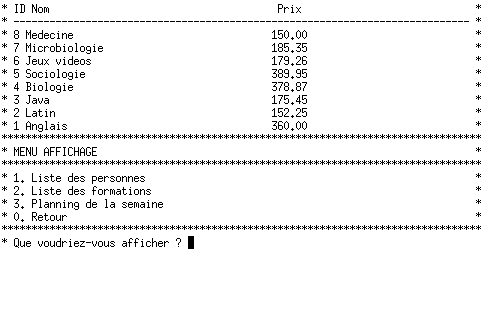
\includegraphics[trim=0 60 0 0, clip, scale=0.8]{images/04.png.png}
\end{figure}
Affiche l'ID, le nom et le prix de chaque formation disponible dans la base de données sous la forme d'une liste.

\newpage
\subsubsection{Planning de la semaine}
\begin{figure}[ht]
  \centering
  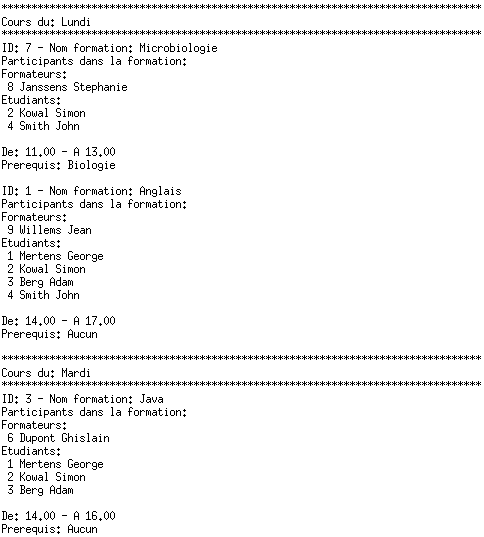
\includegraphics[scale=0.8]{images/05.png.png}
\end{figure}
Les informations sont groupées par jour suivi par le nom de la formation, les différents formateurs, les élèves qui y participent et l'horaiare. Les prérequis pour les formations sont dictées en bas, exemple Biologie est un prérequis pour la formation Microbiologie

\newpage
\subsubsection{Menu ajout}
\begin{figure}[ht]
  \centering
  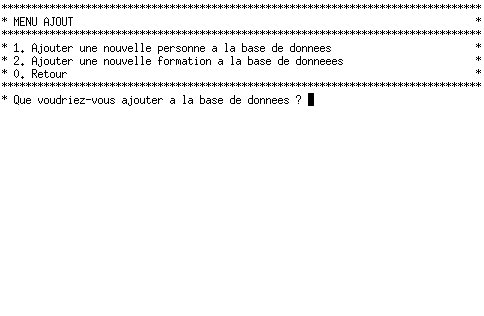
\includegraphics[trim=0 210 0 0, clip, scale=0.8]{images/06.png.png}
\end{figure}
Il est possible d'ajouter une nouvelle personne à la base de données ou ajouter une nouvelle formation à la base de données.

\subsubsection{Ajout d'une personne}
\begin{figure}[ht]
  \centering
  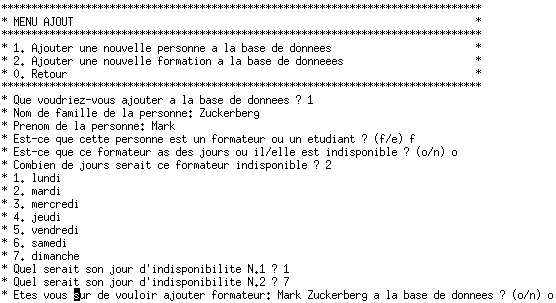
\includegraphics[scale=0.7]{images/07.png.png}
\end{figure}
L'ajout d'une personne se passe de la manière suivante:
\begin{enumerate}
\item Il faut insérer son nom de famille.
\item Il faut insérer son prénom.
\item Il faut insérer son statut (étudiant ou formateur), "f" pour formateur, "e" pour étudiant.
\item Il faut insérer le nombre de jours où le formateur est indisponible.
\item Dépendamment du nombre de jour, il faudra attribuer le jour corréspondant à ceux dans la liste ( 1 - lundi, 2 - mardi, etc\ldots)
\item Il faut confirmer par "o" ou "n" (oui ou non) si l'on souhaite effectivement ajouter la nouvelle personne dans la base de données.
\end{enumerate}

\begin{figure}[ht]
  \centering
  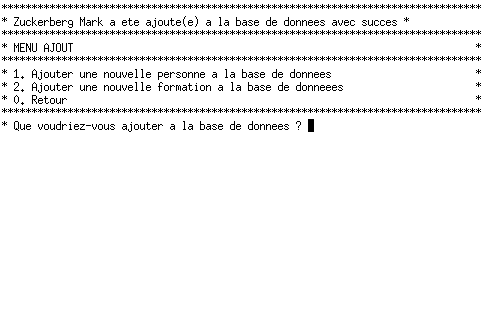
\includegraphics[trim=0 180 0 10, clip, scale=0.8]{images/08.png.png}
\end{figure}
Si la personne a été correctement ajoutée à la base de données, un message de confirmation apparaîtra en haut du menu.\\

\begin{figure}[ht]
  \centering
  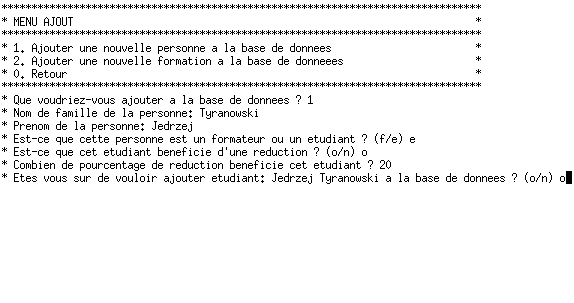
\includegraphics[trim=0 110 0 0, clip, scale=0.7]{images/09.png.png}
\end{figure}
Lorsqu'on ajout un étudiant, il faut indiquer son nom de famille, son prénom et la remise éventuelle.

\begin{figure}[ht]
  \centering
  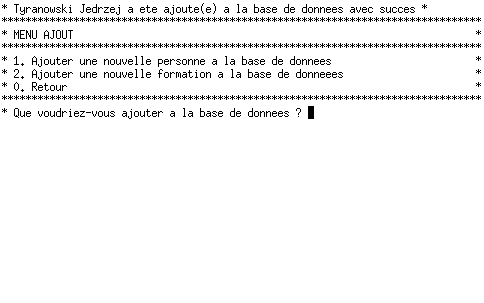
\includegraphics[trim=0 180 0 0, clip, scale=0.8]{images/10.png.png}
\end{figure}
Même message de confirmation pour l'étudiant.

\newpage
\subsubsection{Ajout d'une formation}
\begin{figure}[ht]
  \centering
  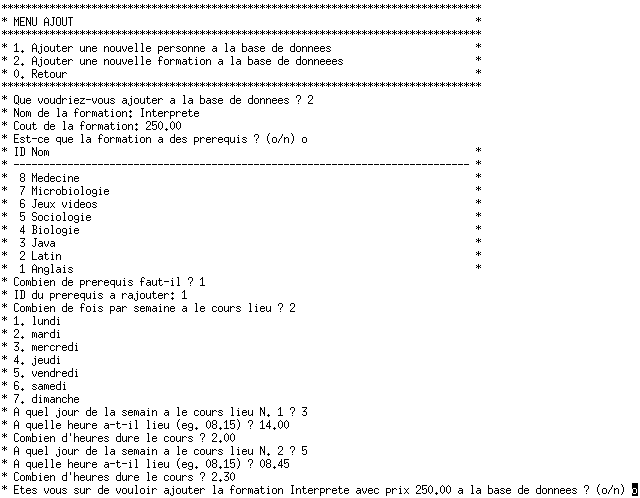
\includegraphics[scale=0.7]{images/11.png.png}
\end{figure}
L'ajout d'une formation se passe de la manière suivante:
\begin{enumerate}
\item Il faut insérer son nom.
\item Il faut insérer son prix.
\item Il faut insérer insérer s'il y a des prérequis ou pas par "o" (oui) et "n" (non).
\item Si oui, il faut insérer le nombre de prérequis et l'ID des formations qui seraient des prérequis.
\item Ensuite il faut dire combiends de fois par semaine la formation a lieu.
\item Dépendamment du nombre de jour, il faudra attribuer le jour corréspondant à ceux dans la liste ( 1 - lundi, 2 - mardi, etc\ldots)
\item Il faut insérer vers quelle heure commence la formation. (En format HH.MM)
\item Il faut insérer combien d'heures dure la formation. (En format HH.MM)
\item Il faut confirmer par "o" ou "n" (oui ou non) si l'on souhaite effectivement ajouter la nouvelle personne dans la base de données.
\end{enumerate}

\begin{figure}[ht]
  \centering
  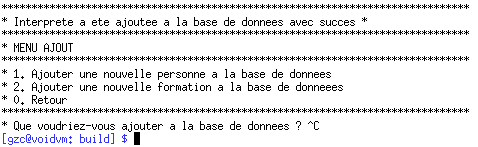
\includegraphics[trim=0 15 10 10, clip, scale=0.8]{images/12.png.png}
\end{figure}
Un message de confirmation apparaîtra au dessus du menu.

\newpage
\subsubsection{Menu attribution}
\begin{figure}[ht]
  \centering
  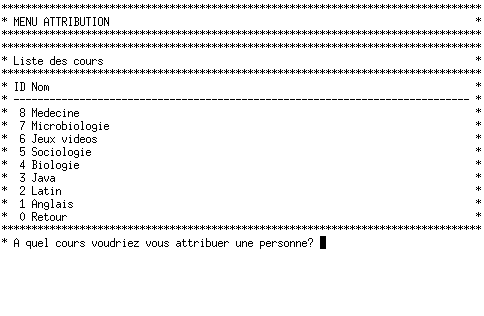
\includegraphics[trim=0 60 0 0, clip, scale=0.8]{images/13.png.png}
\end{figure}
Lorsqu'on rentre dans le menu d'attribution, il faudra séléctionner la formation dans lequelle on souhaite attribuer une personne, formateur ou étudiant.

\newpage
\begin{figure}[ht]
  \centering
  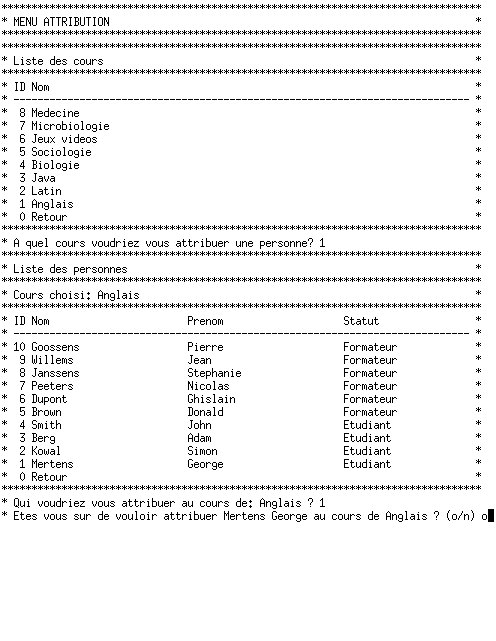
\includegraphics[trim=0 110 0 0, clip, scale=0.8]{images/14.png.png}
\end{figure}
L'attribution à une formation se passe de la manière suivante:
\begin{enumerate}
\item Il faut insérer l'ID de la formation à laquelle on souhaite ajouter un personne quelconque.
\item Il faut insérer l'ID de la personne à rajouter.
\item Il faut confirmer par "o" ou "n" (oui ou non) si l'on souhaite effectivement ajouter la nouvelle personne dans la base de données.
\end{enumerate}

\begin{figure}[ht]
  \centering
  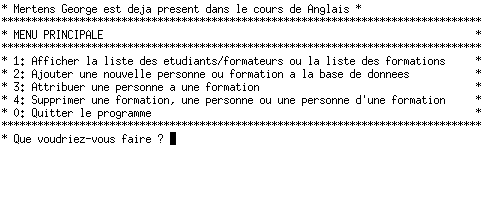
\includegraphics[trim=0 60 0 0, clip, scale=0.8]{images/15.png.png}
\end{figure}
Lors de la réussite de l'attribution de la personne dans la formation, un message de confirmation apparaîtra.

\newpage
\subsubsection{Menu suppression}
\begin{figure}[ht]
  \centering
  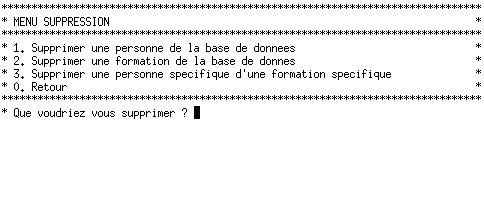
\includegraphics[trim=0 80 0 0, clip, scale=0.8]{images/16.png.png}
\end{figure}

Voici à quoi ressemble l'interface par lequel il est possible de faire des suppressions.
\begin{enumerate}
\item Il est possible de supprimer entièrement une personne de la base de données. Par conséquent, la personne en question disparaîtra des formations aussi.
\item Il est possible de supprimer entièrement une formation de la base de données. Par conséquents, les gens qui particiapaient à la formation en question ne pourront plus y participer.
\item Il est possible de supprimer une personne précise d'une formation précise, bien la formation que la personne apparaîtront dans leurs respectives bases de données, mais ils ne seront plus liés ensemble.
\end{enumerate}

\subsubsection{Suppression d'une personne}
\begin{figure}[ht]
  \centering
  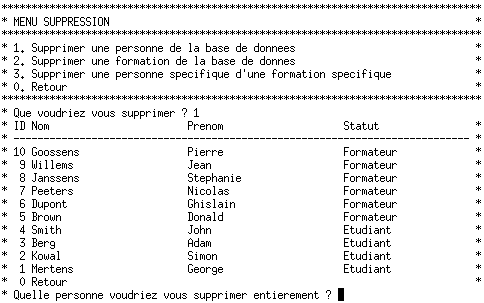
\includegraphics[trim=0 0 0 0, clip, scale=0.8]{images/17.png.png}
\end{figure}
Dans le cas d'une suppression d'une personne de la base de données, il suffit d'insérer l'ID de la personne à supprimer et la personne ne sera plus visible dans aucune formation. Comme toute manipulation, des messages de confirmation apparîtront à la fin de la manipulation.

\newpage
\subsubsection{Suppression d'une formation}
\begin{figure}[ht]
  \centering
  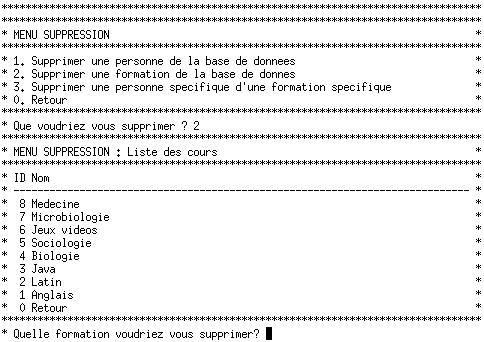
\includegraphics[trim=0 0 0 10, clip, scale=0.8]{images/18.png.png}
\end{figure}
Suivant la même logique que la suppression d'une personne, lors de la suppression d'une formation de la base de données, il suffira d'introduire son ID, appuyer sur Enter et confirmer avec un "o" (oui) ou annuller avec un "n" (non). 

\newpage
\subsubsection{Suppression d'une personne d'une formation spécifique}
\begin{figure}[ht]
  \centering
  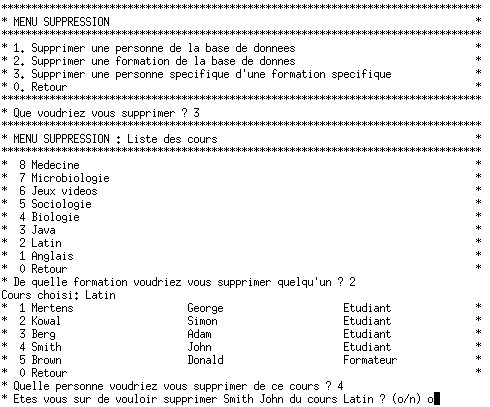
\includegraphics[trim=0 0 0 0, clip, scale=0.7]{images/19.png.png}
\end{figure}
La suppression d'une personne spécifique d'une formation spécifique se passe de la manière suivante:
\begin{enumerate}
\item Il faut insérer l'ID de la formation à partir duquel on souhaite supprimer une personne.
\item Il faut insérer l'ID de la personne à supprimer.
\item Il faut confirmer par "o" ou "n" (oui ou non) si l'on souhaite effectivement ajouter la nouvelle personne dans la base de données.
\end{enumerate}

\begin{figure}[ht]
  \centering
  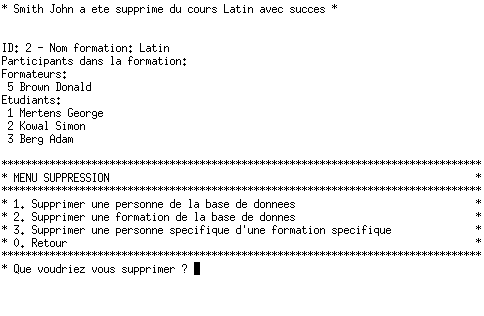
\includegraphics[trim=0 30 0 0, clip, scale=0.7]{images/20.png.png}
\end{figure}

Si la suppression a réussi, un message affichera la réussite de la suppression et affichera le nouvel état de la formation.

\newpage
\section{Code}
\subsection{Structures}
Voici les différentes structures qui ont été utilisée dans la conception du programme:

\begin{lstlisting}[firstnumber=30]
  typedef struct personne
  {
    int id;
    char nom[25];
    char prenom[25];
    int formateur;
    int nb_formations;
    int formations[30];
    int nb_jours_indisponible;
    int jours_indisponible[7];
    int reduction;
    int val_reduction;
  } personne;
\end{lstlisting}

Cette structure sert à stocker les informations qui composent une personne quelconque: étudiant ou formateur.\\
Voici ce que représente chaque partie de la structure:
\begin{itemize}
\item \texttt{int id} : L'identifiant unique de la personne.
\item \texttt{char nom[25]} : Le nom de la personne (25 caractères maximum).
\item \texttt{char prenom[25]} : Le prénom de la personne (25 caractères maximum).
\item \texttt{int formateur} : 1 si la personne est un formateur, 0 si la personne est un étudiant.
\item \texttt{int nb\_formations} : Le nombre de formations auquel la personne participera.
\item \texttt{int formations[30]} : Vecteur qui stockera les idéntifiants des différentes formations auquel la personne participera (On suppose dans une année, une personne ne peut participer qu'à 30 formations maximum).
\item \texttt{int nb\_jours\_indisponible} : Si la personne est un formateur, il se peut qu'il/elle ait des jours d'indisponibilé, cette variable va stocker le nombre de jours où cette personne est indisponile (maximum 7).
\item \texttt{int jours\_indisponibles[7]} : Le vecteur qui stockera les jours auquel le formateur ne sera pas disponible(1 - lundi, 2 - mardi, etc\ldots).
\item \texttt{int reduction} : Si la personne est un étudiant, il se peut qu'il ait une réduction sur son minérval, 1 s'il a droit à une réduction, 0 si pas.
\item \texttt{int val\_reduction} : Le pourcentage de réduction auquel un étudiant à droit.
\end{itemize}

\begin{lstlisting}[firstnumber=51]
  typedef struct noeud_db_personne
  {
    personne *p;
    struct noeud_db_personne *next;
  } noeud_db_personne;
\end{lstlisting}

Cette structure sert à devenir les différents n\oe{}uds qui seront stockés dans la base de donnée, soit la structure \texttt{db\_personne}.
Voici ce qui représent chaque partie de la structure:
\begin{itemize}
\item \texttt{personne *p} : Le pointeur de la personne qui sera stocké dans ce n\oe{}ud lors de sa création.
\item \texttt{struct noeud\_db\_personne *next} : qui contiendra le tête lors qu'on créera un nouveau n\oe{}ud, sinon \texttt{NULL}.
\end{itemize}

\begin{lstlisting}[firstnumber=63]
  typedef struct db_personne
  {
    noeud_db_personne *head;
  } db_personne;
\end{lstlisting}

Cette structure sert à contenir tous les différentes n\oe{}uds \texttt{noeud\_db\_personne}. C'est à partir de cette structure que l'on stockera les différentes n\oe{}uds qui eux-mêmes stockeront leurs personnes respectives.
\begin{itemize}
\item \texttt{noeud\_db\_personne *head} : La tête de la liste chaînée qui stockera toutes les personnes.
\end{itemize}

\begin{lstlisting}[firstnumber=73]
  typedef struct noeud_formation
  {
    personne *p;
    struct noeud_formation *next;
  } noeud_formation;
\end{lstlisting}

Cette structure va stocker les différentes personnes qui participeront à une formation spécifique.
\begin{itemize}
\item \texttt{personne *p} : La personne qui participera à la formation.
\item \texttt{struct noeud\_formation *next} : Le n\oe{}ud de pour la prochaine personne qui sera stockée.
\end{itemize}

\begin{lstlisting}[firstnumber=94]
  typedef struct formation
  {
    int id;
    char nom[40];
    float prix;
    int nb_jours;
    int jours[7];
    float heures[24];
    float durees[10];
    int nb_prerequis;
    int prerequis[10];
    noeud_formation *head;
  } formation;
\end{lstlisting}

Cette structure sert à stocker toutes les informations qui composent une formations.
Voici ce que chaque partie représente:
\begin{itemize}
\item \texttt{int id} : L'identifiant unique de la formation.
\item \texttt{char nom[40]} : Le nom de la formation (40 caractères maximum).
\item \texttt{float prix} : Le coût de la formation.
\item \texttt{int nb\_jours} : Le nombre de jours par semaine où cette formation a lieu.
\item \texttt{int jours[7]} : Vecteur contenant les jours où la formation a lieu.
\item \texttt{float heures[24]} : Le nombre d'heures du début de la formation.
\item \texttt{float durees[10]} : Les différentes durées de la formation lors de la semaine.
\item \texttt{int nb\_prerequis} : Le nombre de prérequis pour avoir accès à cette formation.
\item \texttt{int prerequis[10]} : Vecteur contenant les identifiants des formations qui seraient des prérequis.
\item \texttt{noeud\_formation *head} : Étant donné qu'une formation stocke des personnes, elle-même est une liste chaînée qui stockera un nombre indéterminé de participants.
\end{itemize}

\begin{lstlisting}[firstnumber=115]
  typedef struct noeud_db_formation
  {
    formation *f;
    struct noeud_db_formation *next;
  } noeud_db_formation;
\end{lstlisting}

Cette structure suit la même logique que la structure \texttt{noeud\_db\_personne}. Elle sert à stocker les différentes formations, qui eux-mêmes stockeront les personnes à leurs tour.
\begin{itemize}
\item \texttt{formation *f} : La formation qui sera stockée dans la base de données.
\item \texttt{struct noeud\_db\_formation *next} : La prochaine formation qui sera stockée dans la base de données. \texttt{NULL} si pas de prochaine formation.
\end{itemize}

\begin{lstlisting}[firstnumber=127]
  typedef struct db_formation
  {
    noeud_db_formation *head;
  } db_formation;
\end{lstlisting}

Cette structure aussi suit la même logique que la structure \texttt{db\_formation}. Elle sert de tête pour la la liste chaînée et c'est à partir de cette structure-ci que l'on démarrera les différentes interactions avec la base de données des formations.
\begin{itemize}
\item \texttt{noeud\_db\_formation *head} : La tête de la liste chaînée qui stockera les différentes formations.
\end{itemize}

Pourquoi avons-nous choisi cette approche ? Principalement car on ne voulait pas stocker les différentes personnes et les différentes formations dans des vecteurs. On ne voulait pas qu'il y ait un nombre prédéfini de personnes et un nombre prédéfini de formations, on s'est donc fiés aux listes chaînées. Et c'est pourquoi maintenant il est possible de stocker autant de formations que la \acrshort{ram} nous permet ainsi que de stocker autant de formations que la \acrshort{ram} nous permet.

\newpage
\subsection{Fonctions}
\subsubsection{Fonctions qui créent des n\oe{}ds}
Voici les différentes fonctions que l'on a du créer pour le bon fonctionnement du programme:
\begin{lstlisting}[firstnumber=144]
  personne *creer_personne( char nom[], char prenom[], int formateur );
\end{lstlisting}

Cette fonction sert à créer un pointeur qui permettra d'initialiser les différentes informations présentes dans la structure \texttt{personne}. Lors de l'initialisation d'une personne, on n'aura besoin que du nom de famille de la personne, son prenom et s'il/elle est un formateur ou pas. Le reste des informations est manipulé par la suite lors des différentes interactions.

\begin{lstlisting}[firstnumber=168]
  db_personne *creer_db_personne();
\end{lstlisting}

Cette fonction sert à initialiser le pointer \texttt{noeud\_db\_personne *head} dans la structure \texttt{db\_personne} à \texttt{NULL}, afin que l'on puisse commencer à faire des manipulations avec cette structure.

\begin{lstlisting}[firstnumber=303]
  formation *creer_formation( char nom[], float prix );
\end{lstlisting}

Cette fonction sert à créer un pointeur qui permettra d'initialiser les différentes informations présentes dans la structure \texttt{formation}. Lors de l'initialisation d'une formation, on n'aura besoin que du nom de la formation et de son prix. Le reste des informations est manipulé par la suite lors des différentes interactions.

\begin{lstlisting}[firstnumber=442]
  db_formation *creer_db_formation();
\end{lstlisting}

Cette fonction sert à initialiser le pointer \texttt{noeud\_db\_formation *head} dans la structure \texttt{db\_formation} à \texttt{NULL}, afin que l'on puisse commencer à faire des manipulations avec cette structure.

\subsubsection{Fonctions qui affichent des listes chaînées}

\begin{lstlisting}[firstnumber=157]
  void afficher_personne( personne *p );
\end{lstlisting}

Cette fonction sert à afficher les informations de base qui caractérisent une \textbf{personne}. De manière générale, son identifiant, son nom de famille, son prénom et s'il est formateur ou étudiant.

\begin{lstlisting}[firstnumber=257]
  void afficher_db_personne( db_personne *db );
\end{lstlisting}

Cette fonction parcourt l'entièreté de la base de données \texttt{db\_personne *db}. Tant que la tête n'est pas \texttt{NULL}, on affichera les informations que l'on souhaite afficher de chaque personne présente dans la base de données.

\begin{lstlisting}[firstnumber=408]
  void afficher_formation( formation *f );
\end{lstlisting}

Cette fonction sert à afficher les informations de base qui caractérisent une \textbf{formation}. De manière générale, son identifiant, son nom, son prix, ainsi que les personnes qui y participent.

\begin{lstlisting}[firstnumber=559]
  void afficher_db_formation( db_formation *dbf );
\end{lstlisting}

Cette fonction parcourt l'entièreté de la base de données \texttt{db\_formation *dbf}. Tant que la tête n'est pas \texttt{NULL}, on affichera les informations que l'on souhaite afficher de chaque formation présente dans la base de données.

\subsubsection{Fonctions qui ajoutent un n\oe{}ud à une liste chaînée}

\begin{lstlisting}[firstnumber=187]
  void ajouter_db_personne( db_personne *db, personne *p );
\end{lstlisting}

Cette fonction sert à initialiser un pointeur \texttt{noeud\_db\_personne *ndb} qui stockera \texttt{personne *p} dans la base de données \texttt{db\_personne *db}. Ici, l'ajout dans la liste chaînée à lieu par le mécanisme suivant:
\begin{enumerate}
\item On initialise le noeud temporaire que l'on ajoutera à la base de données.
\item On associe \texttt{p} au pointeur \texttt{p} présent dans la structure \texttt{noeud\_db\_personne}.
\item On initialise le prochain n\oe{}ud de la liste \texttt{*next} à NULL.
\item Si la tête \texttt{*head} de la base de donnée est \texttt{NULL}, alors la tête devient le nouveau n\oe{}ud. On arrête la fonction d'ajout là.
\item Sinon, on fait une copie de la tête dans le n\oe{}ud \texttt{*next} que l'on avait initialisé à \texttt{NULL}.
\item On déclare la tête comme étant le n\oe{}ud temporaire que l'on a initialisé.
\end{enumerate}

\begin{lstlisting}[firstnumber=322]
  int ajouter_formation( formation *f, personne *p );
\end{lstlisting}

Cette fonction sert à initialiser un pointeur \texttt{noeud\_formation *nf} qui stockera \texttt{personne *p} qui participera dans \texttt{formation *f}. Ici, l'ajout dans la liste chaînée à lieu par le mécanisme suivant:
\begin{enumerate}
\item On initialise le noeud temporaire que l'on ajoutera dans la formation.
\item On associe \texttt{p} au pointeur \texttt{p} présent dans la structure \texttt{noeud\_formation}.
\item On initialise le prochain n\oe{}ud de la liste \texttt{*next} à NULL.
\item Si la tête \texttt{*head} de la formation est \texttt{NULL}, alors la tête devient le nouveau n\oe{}ud. On arrête la fonction d'ajout là.
\item Sinon, on fait une copie de la tête dans le n\oe{}ud \texttt{*next} que l'on avait initialisé à \texttt{NULL}.
\item On déclare la tête comme étant le n\oe{}ud temporaire que l'on a initialisé.
\end{enumerate}

\begin{lstlisting}[firstnumber=461]
  void ajouter_db_formation( db_formation *db, formation *f );
\end{lstlisting}

Cette fonction sert à initialiser un pointeur \texttt{noeud\_db\_formation *ndb} qui stockera \texttt{formation *f} dans la base de données \texttt{db\_formation *db}. Ici, l'ajout dans la liste chaînée à lieu par le mécanisme suivant:
\begin{enumerate}
\item On initialise le noeud temporaire que l'on ajoutera à la base de données.
\item On associe \texttt{f} au pointeur \texttt{f} présent dans la structure \texttt{noeud\_db\_formation}.
\item On initialise le prochain n\oe{}ud de la liste \texttt{*next} à NULL.
\item Si la tête \texttt{*head} de la base de donnée est \texttt{NULL}, alors la tête devient le nouveau n\oe{}ud. On arrête la fonction d'ajout là.
\item Sinon, on fait une copie de la tête dans le n\oe{}ud \texttt{*next} que l'on avait initialisé à \texttt{NULL}.
\item On déclare la tête comme étant le n\oe{}ud temporaire que l'on a initialisé.
\end{enumerate}

\subsubsection{Fonctions qui suppriment un n\oe{}ud d'une liste chaînée}

\begin{lstlisting}[firstnumber=216]
  int supprimer_db_personne( db_personne *dbp, int id );
\end{lstlisting}

Cette fonction sert à supprimer une personne de la base de données à partir de son identifiant. La démarche faite dans cette fonction est la suivant:
\begin{enumerate}
\item On vérife que la tête de la base de données \texttt{dbp->head} ne soit pas \texttt{NULL}, si oui, on arrête la fonction.
\item On vérifie si le premier élément de la liste correspond à l'\texttt{id} de la personne que l'on souhaite supprimer.
\item Si oui:
  \begin{enumerate}
  \item On crée un n\oe{}ud temporaire qui stockera la personne suivante dans la liste.
  \item On libére l'espace mémoire occupé par head avec la fonction \texttt{free(dbp->head)}.
  \item On attribue à \texttt{dbp->head} le n\oe{}ud temporaire que l'on avait créé.
  \item On arrête la fonction.
  \end{enumerate}
\item Sinon, on parcourt l'entièreté de la liste jusqu'au moment où l'on trouve la personne qui a le même \texttt{id} que l'\texttt{id} en paramètre.
\item Si on le trouve, on pivote l'élément qui suit vers l'élément que l'on vient de supprimer.
\item On arrête la fonction, si réussite, on obtient 1, si pas, on obtient 0.
\end{enumerate}

\begin{lstlisting}[firstnumber=361]
  int supprimer_personne_de_formation( formation *f, int id );
\end{lstlisting}

Cette fonction sert à supprimer une personne de la fonction à partir de son identifiant. La démarche faite dans cette fonction est la suivant:
\begin{enumerate}
\item On vérife que la tête de la fonction \texttt{f->head} ne soit pas \texttt{NULL}, si oui, on arrête la fonction.
\item On vérifie si le premier élément de la liste correspond à l'\texttt{id} de la personne que l'on souhaite supprimer.
\item Si oui:
  \begin{enumerate}
  \item On crée un n\oe{}ud temporaire qui stockera la personne suivante dans la liste.
  \item On libére l'espace mémoire occupé par head avec la fonction \texttt{free(f->head)}.
  \item On attribue à \texttt{f->head} le n\oe{}ud temporaire que l'on avait créé.
  \item On arrête la fonction.
  \end{enumerate}
\item Sinon, on parcourt l'entièreté de la liste jusqu'au moment où l'on trouve la personne qui a le même \texttt{id} que l'\texttt{id} en paramètre.
\item Si on le trouve, on pivote l'élément qui suit vers l'élément que l'on vient de supprimer.
\item On arrête la fonction, si réussite, on obtient 1, si pas, on obtient 0.
\end{enumerate}

\begin{lstlisting}[firstnumber=490]
  int supprimer_db_formation( db_formation *dbf, int id );
\end{lstlisting}

Cette fonction sert à supprimer une formation de la base de données à partir de son identifiant. La démarche faite dans cette fonction est la suivant:
\begin{enumerate}
\item On vérife que la tête de la base de données \texttt{dbf->head} ne soit pas \texttt{NULL}, si oui, on arrête la fonction.
\item On vérifie si le premier élément de la liste correspond à l'\texttt{id} de la formation que l'on souhaite supprimer.
\item Si oui:
  \begin{enumerate}
  \item On crée un n\oe{}ud temporaire qui stockera la formation suivante dans la liste.
  \item On libére l'espace mémoire occupé par head avec la fonction \texttt{free(dbf->head)}.
  \item On attribue à \texttt{dbf->head} le n\oe{}ud temporaire que l'on avait créé.
  \item On arrête la fonction.
  \end{enumerate}
\item Sinon, on parcourt l'entièreté de la liste jusqu'au moment où l'on trouve la formation qui a le même \texttt{id} que l'\texttt{id} en paramètre.
\item Si on le trouve, on pivote l'élément qui suit vers l'élément que l'on vient de supprimer.
\item On arrête la fonction, si réussite, on obtient 1, si pas, on obtient 0.
\end{enumerate}

\subsubsection{Fonctions qui servent de \texttt{getter()}}

\begin{lstlisting}[firstnumber=275]
  personne *get_personne( db_personne *db, char nom[], char prenom[], int formateur );
\end{lstlisting}

Cette fonction renvoie \texttt{NULL} si une personne d'un nom spécifique, d'un prénom spécifique, et s'il est formateur ou étudiant n'existe pas dans la base de données \texttt{db\_personne *db}. Sinon, la fonction retourne la personne trouvée.

\begin{lstlisting}[firstnumber=532]
  formation *get_formation( db_formation *dbf, char nom_formation[] );
\end{lstlisting}

Cette fonction renvoie \texttt{NULL} si une formation avec un nom spécifique n'existe pas dans la base de données \texttt{db\_formation *dbf}. Sinon, la fonction retourne la formation trouvée.

\subsubsection{Fonctions qui affiches les différentes parties du menu interactif}
les fonctions ci-dessous ne servent qu'à affichier les différentes parties du menu interactif. Elle ne font aucune manipulation particulière autre qu'affichier du texte. Le \texttt{main()} est la seule fonction qui lit les données et les initialise dans la base de données avant que le menu soit affiché.

\begin{lstlisting}[firstnumber=618]
  void menu_creer_formation( db_formation *f );
\end{lstlisting}

\begin{lstlisting}[firstnumber=793]
  void menu_creer_personne( db_personne *p );
\end{lstlisting}

\begin{lstlisting}[firstnumber=953]
  int menu_creer( db_formation *f, db_personne *p );
\end{lstlisting}

\begin{lstlisting}[firstnumber=990]
  void menu_ajouter_formation( db_formation *f, db_personne *p );
\end{lstlisting}

\begin{lstlisting}[firstnumber=1103]
  void menu_supprimer_personne( db_formation *dbf, db_personne *dbp );
\end{lstlisting}

\begin{lstlisting}[firstnumber=1182]
  void menu_supprimer_formation( db_formation *dbf, db_personne *dbp );
\end{lstlisting}

\begin{lstlisting}[firstnumber=1271]
  int menu_supprimer_personne_de_formation( db_formation *dbf );
\end{lstlisting}

\begin{lstlisting}[firstnumber=1396]
  int menu_supprimer( db_formation *dbf, db_personne *dbp );
\end{lstlisting}

\begin{lstlisting}[firstnumber=1436]
  int menu_affichage( db_formation *f, db_personne *p );
\end{lstlisting}

\begin{lstlisting}[firstnumber=1489]
  int ecrire_planning( db_formation *dbf );
\end{lstlisting}

\begin{lstlisting}[firstnumber=1572]
  int menu( db_formation *f, db_personne *p );
\end{lstlisting}

\begin{lstlisting}[firstnumber=1704]
  int main( void );
\end{lstlisting}

\subsubsection{Entièreté du code}
\begin{lstlisting}
#include <ctype.h>
#include <stdio.h>
#include <string.h>
#include <stdlib.h>

#if defined(WIN32) || defined(_WIN32) || defined(__WIN32__) || defined(__NT__)
char *clear = "cls";
#elif __unix__ || __APPLE__ && __MACH__
char *clear = "clear";
#endif

/*****************************************************************************/
/*                                     STRUCTS                               */
/*
 * int id : L'identifiant unique de la personne
 * char nom[25] : Le nom de la personne (25 caracteres maximum)
 * char prenom[25] : Le prenom de la personne (25 caracteres maximum)
 * int formateur : 1 si la personne est un formateur, 0 si la personne est un etudiant
 * int nb_formations : Le nombre de formations auquel la personne participera
 * int formations[30] : Vecteur qui stockera les identifiants des differentes formations auquel la personne participera
 * (On suppose dans une annee, une personne ne peut participer qu'a 30 formations maximum)
 * int nb_jours_indisponible : Si la personne est un formateur, il se peut qu'il/elle ait des jours d'indisponibile,
 * cette variable va stocker le nombre de jours ou cette personne est indisponile (maximum 7)
 * int jours_indisponibles[7] : Le vecteur qui stockera les jours auquel le formateur ne sera pas disponible
 * (1 - lundi, 2 - mardi, etc...)
 * int reduction : Si la personne est un etudiant, il se peut qu'il ait une reduction sur son minerval,
 * 1 s'il a droit a une reduction, 0 si pas
 * int val_reduction : Le pourcentage de reduction auquel un etudiant a droit
 */
typedef struct personne
{
    int id;
    char nom[25];
    char prenom[25];
    int formateur;
    int nb_formations;
    int formations[30];
    int nb_jours_indisponible;
    int jours_indisponible[7];
    int reduction;
    int val_reduction;
} personne;

/*
 * Cette structure sert a devenir les differents noeuds qui seront stockes dans la base de donnee,
 * soit la structure db_personne.
 * Voici ce qui represent chaque partie de la structure:
 * personne *p : Le pointeur de la personne qui sera stocke dans ce nud lors de sa creation.
 * struct noeud_db_personne *next : qui contiendra le tete lors qu'on creera un nouveau nud, sinon NULL.
 */
typedef struct noeud_db_personne
{
    personne *p;
    struct noeud_db_personne *next;
} noeud_db_personne;

/*
 * Cette structure sert a contenir tous les differentes noeuds noeud_db_personne.
 * C'est a partir de cette structure que l'on stockera les differentes noeuds qui eux-memes stockeront
 * leurs personnes respectives.
 * noeud_db_personne *head : La tete de la liste chainee qui stockera toutes les personnes.
 */
typedef struct db_personne
{
    noeud_db_personne *head;
} db_personne;

/*
 * Cette structure va stocker les differentes personnes qui participeront a une formation specifique.
 * personne *p : La personne qui participera a la formation.
 * struct noeud_formation *next : Le noeud de pour la prochaine personne qui sera stockee.
 */
typedef struct noeud_formation
{
    personne *p;
    struct noeud_formation *next;
} noeud_formation;

/*
 * Cette structure sert a stocker toutes les informations qui composent une formations.
 * Voici ce que chaque partie represente:
 * int id : L'identifiant unique de la formation.
 * char nom[40] : Le nom de la formation (40 caracteres maximum).
 * float prix : Le cout de la formation.
 * int nb_jours : Le nombre de jours par semaine ou cette formation a cours.
 * int jours[7] : Vecteur contenant les jours ou la formation a cours.
 * float heures[24] : Le nombre d'heures du debut de la formation.
 * float durees[10] : Les differentes durees du cours lors de la semaine.
 * int nb_prerequis : Le nombre de prerequis pour avoir acces a cette formation.
 * int prerequis[10] : Vecteur contenant les identifiants des formations qui seraient des prerequis.
 * noeud_formation *head : Etant donne qu'une formation stocke des personnes,
 * elle-meme est une liste chainee qui stockera un nombre indetermine de participants.
 */
typedef struct formation
{
    int id;
    char nom[40];
    float prix;
    int nb_jours;
    int jours[7];
    float heures[24];
    float durees[10];
    int nb_prerequis;
    int prerequis[10];
    noeud_formation *head;
} formation;

/*
 * Cette structure suit la meme logique que la structure noeud_db_personne.
 * Elle sert a stocker les differentes formations, qui eux-memes stockeront les personnes a leurs tour.
 * formation *f : La formation qui sera stockee dans la base de donnees.
 * struct noeud_db_formation *next : La prochaine formation qui sera stockee dans la base de donnees.
 * NULL si pas de prochaine formation.
 */
typedef struct noeud_db_formation
{
    formation *f;
    struct noeud_db_formation *next;
} noeud_db_formation;

/*
 * Cette structure aussi suit la meme logique que la structure db_formation.
 * Elle sert de tete pour la la liste chainee et c'est a partir de cette structure-ci que l'on demarrera
 * les differentes interactions avec la base de donnees des formations.
 * noeud_db_formation *head : La tete de la liste chainee qui stockera les differentes formations.
 */
typedef struct db_formation
{
    noeud_db_formation *head;
} db_formation;

/*                                    FIN STRUCTS                            */
/*****************************************************************************/

/*****************************************************************************/
/*                                    PERSONNE                               */
/*
 * Cette fonction sert a creer un pointeur qui permettra d'initialiser les differentes informations presentes
 * dans la structure personne.
 * Lors de l'initialisation d'une personne, on n'aura besoin que du nom de famille de la personne,
 * son prenom et s'il/elle est un formateur ou pas.
 * Le reste des informations est manipule par la suite lors des differentes interactions.
 */
personne *creer_personne( char nom[], char prenom[], int formateur )
{
    personne *e = ( personne * ) calloc( sizeof( personne ), sizeof( personne ) );
    strcpy( e->nom, nom );
    strcpy( e->prenom, prenom );
    e->formateur = formateur;
    return e;
}

/*
 * Cette fonction sert a afficher les informations de base qui caracterisent une personne.
 * De maniere generale, son identifiant, son nom de famille, son prenom et s'il est formateur ou etudiant.
 */
void afficher_personne( personne *p )
{
    personne *tmp = p;
    printf( "* %2d %-25s %-25s %-10s            *\n",
            tmp->id, tmp->nom, tmp->prenom, tmp->formateur ? "Formateur" : "Etudiant" );
}

/*
 * Cette fonction sert a initialiser le pointer noeud_db_personne *head dans la structure db_personne a NULL,
 * afin que l'on puisse commencer a faire des manipulations avec cette structure.
 */
db_personne *creer_db_personne()
{
    db_personne *db = ( db_personne * ) calloc( sizeof( db_personne ), sizeof( db_personne ) );
    db->head = NULL;
    return db;
}

/*
 * Cette fonction sert a initialiser un pointeur noeud_db_personne *ndb qui stockera personne *p
 * dans la base de donnees db_personne *db.
 * Ici, l'ajout dans la liste chainee a lieu par le mecanisme suivant:
 * On initialise le noeud temporaire que l'on ajoutera a la base de donnees.
 * On associe p au pointeur p present dans la structure noeud_db_personne.
 * On initialise le prochain noeud de la liste *next a NULL.
 * Si la tete *head de la base de donnee est NULL, alors la tete devient le nouveau noeud.
 * On arrete la fonction d'ajout la.
 * Sinon, on fait une copie de la tete dans le noeud *next que l'on avait initialise a NULL.
 * On declare la tete comme etant le noeud temporaire que l'on a initialise.
 */
void ajouter_db_personne( db_personne *db, personne *p )
{
    noeud_db_personne *ndb = ( noeud_db_personne * ) calloc( sizeof( noeud_db_personne ), sizeof( noeud_db_personne ) );
    ndb->p = p;
    ndb->next = NULL;
    if( db->head == NULL )
    {
        db->head = ndb;
        return;
    }
    ndb->next = db->head;
    db->head = ndb;
}

/*
 * Cette fonction sert a supprimer une personne de la base de donnees a partir de son identifiant.
 * La demarche faite dans cette fonction est la suivant:
 * On verife que la tete de la base de donnees dbp->head ne soit pas NULL, si oui, on arrete la fonction.
 * On verifie si le premier element de la liste correspond a l'id de la personne que l'on souhaite supprimer.
 * Si oui:
 * On cree un noeud temporaire qui stockera la personne suivante dans la liste.
 * On libere l'espace memoire occupe par head avec la fonction free(dbp->head).
 * On attribue a dbp->head le noeud temporaire que l'on avait cree.
 * On arrete la fonction.
 * Sinon, on parcourt l'entierete de la liste jusqu'au moment ou l'on trouve la personne qui a le meme id que
 * l'id en parametre.
 * Si on le trouve, on pivote l'element qui suit vers l'element que l'on vient de supprimer.
 * On arrete la fonction, si reussite, on obtient 1, si pas, on obtient 0.
 */
int supprimer_db_personne( db_personne *dbp, int id )
{
    noeud_db_personne *ndbp = dbp->head;
    if( ndbp == NULL )
    {
        return 0;
    }
    noeud_db_personne *tmp = NULL;
    if( ndbp->p->id == id )
    {
        tmp = dbp->head->next;
        free( dbp->head );
        dbp->head = tmp;
        return 1;
    }
    while( ndbp != NULL )
    {
        if( ndbp->next == NULL )
        {
            if( ndbp->p->id == id )
            {
                return 1;
            }
            return 0;
        }
        if( ndbp->next->p->id == id )
        {
            tmp = ndbp->next;
            ndbp->next = tmp->next;
            free( tmp );
            return 1;
        }
        ndbp = ndbp->next;
    }
    return 0;
}

/*
 * Cette fonction parcourt l'entierete de la base de donnees db_personne *db.Tant que la tete n'est pas NULL,
 * on affichera les informations que l'on souhaite afficher de chaque personne presente dans la base de donnees.
 */
void afficher_db_personne( db_personne *db )
{
    db_personne *tmpdb = db;
    noeud_db_personne *tmpndb = tmpdb->head;
    printf( "* %2s %-25s %-25s %-9s             *\n", "ID", "Nom", "Prenom", "Statut" );
    printf( "* ---------------------------------------------------------------------------- *\n" );
    while( tmpndb != NULL )
    {
        afficher_personne( tmpndb->p );
        tmpndb = tmpndb->next;
    }
}

/*
 * Cette fonction renvoie NULL si une formation avec un nom specifique n'existe pas dans
 * la base de donnees db_formation *dbf.
 * Sinon, la fonction retourne la formation trouvee.
 */
personne *get_personne( db_personne *db, char nom[], char prenom[], int formateur )
{
    db_personne *tmpdb = db;
    noeud_db_personne *tmpndb = tmpdb->head;
    while( tmpndb != NULL )
    {
        if( strcmp( tmpndb->p->nom, nom ) == 0 &&
            strcmp( tmpndb->p->prenom, prenom ) == 0 &&
            tmpndb->p->formateur == formateur )
        {
            return tmpndb->p;
        }
        tmpndb = tmpndb->next;
    }
    return NULL;
}

/*                                 FIN PERSONNE                              */
/*****************************************************************************/

/*****************************************************************************/
/*                                     FORMATION                             */
/*
 * Cette fonction sert a creer un pointeur qui permettra d'initialiser les differentes informations presentes dans
 * la structure formation.
 * Lors de l'initialisation d'une formation, on n'aura besoin que du nom de la formation et de son prix.
 * Le reste des informations est manipule par la suite lors des differentes interactions.
 */
formation *creer_formation( char nom[], float prix )
{
    formation *tmp = ( formation * ) calloc( sizeof( formation), sizeof( formation ) );
    strcpy( tmp->nom, nom );
    tmp->prix = prix;
    tmp->head = NULL;
    return tmp;
}
/*
 * Cette fonction sert a initialiser un pointeur noeud_formation *nf qui stockera personne *p qui participera
 * dans formation *f. Ici,
 * l'ajout dans la liste chainee a lieu par le mecanisme suivant:
 * On initialise le noeud temporaire que l'on ajoutera dans la formation.
 * On associe p au pointeur p present dans la structure noeud_formation.
 * On initialise le prochain noeud de la liste *next a NULL.
 * Si la tete *head de la formation est NULL, alors la tete devient le nouveau noeud. On arrete la fonction d'ajout la.
 * Sinon, on fait une copie de la tete dans le noeud *next que l'on avait initialise a NULL.
 * On declare la tete comme etant le noeud temporaire que l'on a initialise.
 */
int ajouter_formation( formation *f, personne *p )
{
    noeud_formation *nf = ( noeud_formation * ) calloc( sizeof( noeud_formation ), sizeof( noeud_formation) );
    nf->p = p;
    nf->next = NULL;
    if( f->head == NULL )
    {
        f->head = nf;
        return 1;
    }
    noeud_formation *tmpnf = f->head;
    while( tmpnf != NULL )
    {
        if( tmpnf->p->id == p->id )
        {
            return 0;
        }
        tmpnf = tmpnf->next;
    }
    nf->next = f->head;
    f->head = nf;
    return 1;
}

/*
 * Cette fonction sert a supprimer une personne de la fonction a partir de son identifiant.
 * La demarche faite dans cette fonction est la suivant:
 * On verife que la tete de la fonction f->head ne soit pas NULL, si oui, on arrete la fonction.
 * On verifie si le premier element de la liste correspond a l'id de la personne que l'on souhaite supprimer.
 * Si oui:
 * On cree un noeud temporaire qui stockera la personne suivante dans la liste.
 * On libere l'espace memoire occupe par head avec la fonction free(f->head).
 * On attribue a f->head le noeud temporaire que l'on avait cree.
 * On arrete la fonction.
 * Sinon, on parcourt l'entierete de la liste jusqu'au moment ou l'on trouve la personne
 * qui a le meme id que l'id en parametre.
 * Si on le trouve, on pivote l'element qui suit vers l'element que l'on vient de supprimer.
 * On arrete la fonction, si reussite, on obtient 1, si pas, on obtient 0.
 */
int supprimer_personne_de_formation( formation *f, int id )
{
    formation *tmpf = f;
    noeud_formation *tmp = NULL;
    if( f == NULL )
    {
        printf( "Formation pas trouvee\n" );
        return 0;
    }
    noeud_formation *headf = tmpf->head;
    if( headf == NULL )
    {
        return 0;
    }
    if( f->head->p->id == id )
    {
        tmp = f->head->next;
        free( f->head );
        f->head = tmp;
        return 1;
    }
    while( headf != NULL )
    {
        if( headf->next == NULL )
        {
            if( headf->p->id == id )
            {
                return 1;
            }
            return 0;
        }
        if( headf->next->p->id == id )
        {
            tmp = headf->next;
            headf->next = tmp->next;
            free( tmp );
            return 1;
        }
        headf = headf->next;
    }
    return 0;
}

/*
 * Cette fonction sert a afficher les informations de base qui caracterisent une formation.
 * De maniere generale, son identifiant, son nom, son prix, ainsi que les personnes qui y participent.
 */
void afficher_formation( formation *f )
{
    formation *tmp = f;
    noeud_formation *tmpnf = tmp->head;
    printf( "ID: %d - Nom formation: %s\n", tmp->id, tmp->nom );
    printf( "Participants dans la formation:\n" );
    printf( "Formateurs:\n" );
    while( tmpnf != NULL )
    {
        if( tmpnf->p->formateur == 1 )
        {
            printf( "%2d %s %s", tmpnf->p->id, tmpnf->p->nom, tmpnf->p->prenom );
            if( tmpnf != NULL ) printf( "\n" );
        }
        tmpnf = tmpnf->next;
    }
    tmpnf = tmp->head;
    printf( "Etudiants:\n" );
    while( tmpnf != NULL )
    {
        if( tmpnf->p->formateur == 0 )
        {
            printf( "%2d %s %s", tmpnf->p->id, tmpnf->p->nom, tmpnf->p->prenom );
            if( tmpnf != NULL ) printf( "\n" );
        }
        tmpnf = tmpnf->next;
    }
    printf( "\n" );
}

/*
 * Cette fonction sert a initialiser le pointer noeud_db_formation *head dans la structure db_formation a NULL,
 * afin que l'on puisse commencer a faire des manipulations avec cette structure.
 */
db_formation *creer_db_formation()
{
    db_formation *db = ( db_formation * ) calloc( sizeof( db_formation ), sizeof( db_formation ) );
    db->head = NULL;
    return db;
}

/*
 * Cette fonction sert a initialiser un pointeur noeud_db_formation *ndb qui stockera formation *f dans
 * la base de donnees db_formation *db.
 * Ici, l'ajout dans la liste chainee a lieu par le mecanisme suivant:
 * On initialise le noeud temporaire que l'on ajoutera a la base de donnees.
 * On associe f au pointeur f present dans la structure noeud_db_formation.
 * On initialise le prochain noeud de la liste *next a NULL.
 * Si la tete *head de la base de donnee est NULL, alors la tete devient le nouveau noeud.
 * On arrete la fonction d'ajout la.
 * Sinon, on fait une copie de la tete dans le noeud *next que l'on avait initialise a NULL.
 * On declare la tete comme etant le noeud temporaire que l'on a initialise.
 */
void ajouter_db_formation( db_formation *db, formation *f )
{
    noeud_db_formation *ndb = ( noeud_db_formation * ) calloc( sizeof( noeud_db_formation ), sizeof( noeud_db_formation ) );
    ndb->f = f;
    ndb->next = NULL;
    if( db->head == NULL )
    {
        db->head = ndb;
        return;
    }
    ndb->next = db->head;
    db->head = ndb;
}

/*
 * Cette fonction sert a supprimer une formation de la base de donnees a partir de son identifiant.
 * La demarche faite dans cette fonction est la suivant:
 * On verife que la tete de la base de donnees dbf->head ne soit pas NULL, si oui, on arrete la fonction.
 * On verifie si le premier element de la liste correspond a l'id de la formation que l'on souhaite supprimer.
 * Si oui:
 * On cree un noeud temporaire qui stockera la formation suivante dans la liste.
 * On libere l'espace memoire occupe par head avec la fonction free(dbf->head).
 * On attribue a dbf->head le noeud temporaire que l'on avait cree.
 * On arrete la fonction.
 * Sinon, on parcourt l'entierete de la liste jusqu'au moment ou l'on trouve la formation qui
 * a le meme id que l'id en parametre.
 * Si on le trouve, on pivote l'element qui suit vers l'element que l'on vient de supprimer.
 * On arrete la fonction, si reussite, on obtient 1, si pas, on obtient 0.
 */
int supprimer_db_formation( db_formation *dbf, int id )
{
    noeud_db_formation *tmp = NULL;
    if( dbf->head == NULL )
    {
        return 0;
    }
    if( dbf->head->f->id == id )
    {
        tmp = dbf->head->next;
        free( dbf->head );
        dbf->head = tmp;
        return 1;
    }
    noeud_db_formation *tmpndbf = dbf->head;
    while( tmpndbf != NULL )
    {
        if( tmpndbf->next == NULL )
        {
            if( tmpndbf->f->id == id )
            {
                return 1;
            }
            return 0;
        }
        if( tmpndbf->next->f->id == id )
        {
            tmp = tmpndbf->next;
            tmpndbf->next = tmpndbf->next->next;
            free( tmp );
            return 1;
        }
        tmpndbf = tmpndbf->next;
    }
    return 0;
}

/*
 * Cette fonction renvoie NULL si une formation avec un nom specifique n'existe pas dans
 * la base de donnees db_formation *dbf.
 * Sinon, la fonction retourne la formation trouvee.
 */
formation *get_formation( db_formation *dbf, char nom_formation[] )
{
    db_formation *tmpdbf = dbf;
    noeud_db_formation *tmpndbf = tmpdbf->head;
    while( tmpndbf != NULL )
    {
        if( strcmp( tmpndbf->f->nom, nom_formation ) == 0 )
        {
            return tmpndbf->f;
        }
        tmpndbf = tmpndbf->next;
    }
    return NULL;
}

/*
 * Cette fonction sert a initialiser un pointeur noeud_db_formation *ndb qui stockera formation *f dans
 * la base de donnees db_formation *db.
 * Ici, l'ajout dans la liste chainee a lieu par le mecanisme suivant:
 * On initialise le noeud temporaire que l'on ajoutera a la base de donnees.
 * On associe f au pointeur f present dans la structure noeud_db_formation.
 * On initialise le prochain noeud de la liste *next a NULL.
 * Si la tete *head de la base de donnee est NULL, alors la tete devient le nouveau noeud.
 * On arrete la fonction d'ajout la.
 * Sinon, on fait une copie de la tete dans le noeud *next que l'on avait initialise a NULL.
 * On declare la tete comme etant le noeud temporaire que l'on a initialise.
 */
void afficher_db_formation( db_formation *dbf )
{
    int i;
    db_formation *tmpdbf = dbf;
    noeud_db_formation *tmpndbf = tmpdbf->head;
    char jour[7][9] = { "Lundi", "Mardi", "Mercredi", "Jeudi", "Vendredi", "Samedi", "Dimanche" };
    for( i = 1; i <= 7; i++ )
    {
        tmpndbf = tmpdbf->head;
        printf( "********************************************************************************\n" );
        printf( "Cours du: %s\n", jour[i - 1] );
        printf( "********************************************************************************\n" );
        while( tmpndbf != NULL )
        {
            formation *tmp = tmpndbf->f;
            int j;
            for( j = 0; j < tmp->nb_jours; j++ )
            {
                if( tmp->jours[j] == i )
                {
                    afficher_formation( tmp );
                    printf( "De: %.2f - A %.2f\n", tmp->heures[j], tmp->heures[j] + tmp->durees[j] );
                    printf( "Prerequis: " );
                    if( tmp->nb_prerequis > 0 )
                    {
                        db_formation *tmpdb = dbf;
                        noeud_db_formation *tmp_prereq_ndbf = tmpdb->head;
                        while( tmp_prereq_ndbf != NULL )
                        {
                            formation *tmp_prereq = tmp_prereq_ndbf->f;
                            int k;
                            for( k = 0; k < tmp->nb_prerequis; k++ )
                            {
                                if( tmp->prerequis[k] == tmp_prereq->id )
                                {
                                    printf( "%s ", tmp_prereq->nom );
                                }
                            }
                            tmp_prereq_ndbf = tmp_prereq_ndbf->next;
                        }
                        printf( "\n\n" );
                    }
                    else
                    {
                        printf( "Aucun\n\n" );
                    }
                }
            }
            tmpndbf = tmpndbf->next;
        }
    }
}

/*                             FIN FORMATION                                 */
/*****************************************************************************/

/*****************************************************************************/
/*                           FONCTIONS GENERALES                             */

void menu_creer_formation( db_formation *f )
{
    db_formation *tmpdbf = f;
    int i;
    char nom[40];
    float prix;
    printf( "* Nom de la formation: " );
    fgets( nom, 40, stdin );
    if( strlen( nom ) > 0 && nom[ strlen( nom ) - 1 ] == '\n' )
    {
        nom[ strlen( nom ) - 1 ] = '\0';
    }
    formation *tmp = get_formation( f, nom );
    if( tmp == NULL )
    {
        printf( "* Cout de la formation: " );
        while( scanf( "%f", &prix ) != 1 )
        {
            printf( "* Option %.2f - INVALIDE: Min 0\n", prix );
            printf( "* Cout de la formation: " );
            scanf( "%f", &prix );
            getchar();
        }
        while( prix < 0 )
        {
            printf( "* Option %.2f - INVALIDE: Min 0\n", prix );
            printf( "* Cout de la formation: " );
            scanf( "%f", &prix );
            getchar();
        }
        formation *tmpf = creer_formation( nom, prix );
        if( tmpdbf->head == NULL )
        {
            tmpf->id = 1;
        }
        else
        {
            tmpf->id = tmpdbf->head->f->id + 1;
        }
        char choix_prerequis[4];
        printf( "* Est-ce que la formation a des prerequis ? (o/n) " );
        scanf( "%s", choix_prerequis );
        getchar();
        while( strcmp( choix_prerequis, "o" ) != 0 && strcmp( choix_prerequis, "oui" ) != 0 &&
               strcmp( choix_prerequis, "n" ) != 0 && strcmp( choix_prerequis, "non" ) != 0 )
        {
            printf( "* Options %s - INVALIDE: o pour oui et n pour non s'il vous plait\n", choix_prerequis );
            printf( "* Est-ce que la formation a des prerequis ? (o/n) " );
            scanf( "%s", choix_prerequis );
            getchar();
        }
        if( strcmp( choix_prerequis, "o" ) == 0 || strcmp( choix_prerequis, "oui" ) == 0 )
        {
            noeud_db_formation *tmpndbf = tmpdbf->head;
            printf( "* %2s %-40s                                  *\n", "ID", "Nom" );
            printf( "* ---------------------------------------------------------------------------- *\n" );
            while( tmpndbf != NULL )
            {
                printf( "* %2d %-40s                                  *\n", tmpndbf->f->id, tmpndbf->f->nom );
                tmpndbf = tmpndbf->next;
            }
            tmpndbf = tmpdbf->head;
            int nb_prerequis;
            printf( "* Combien de prerequis faut-il ? " );
            while( scanf( "%d", &nb_prerequis ) != 1 )
            {
                printf( "* Option %d - INVALIDE: Max %d prerequis Min 0\n", nb_prerequis, tmpndbf->f->id );
                printf( "* Combien de prerequis faut-il ? " );
                scanf( "%d", &nb_prerequis );
                getchar();
            }
            getchar();
            while( nb_prerequis > tmpndbf->f->id || nb_prerequis < 0 )
            {
                printf( "* Option %d - INVALIDE: Max %d prerequis Min 0\n", nb_prerequis, tmpndbf->f->id );
                printf( "* Combien de prerequis faut-il ? " );
                scanf( "%d", &nb_prerequis );
                getchar();
            }
            tmpf->nb_prerequis = nb_prerequis;
            for( i = 0; i < nb_prerequis; i++ )
            {
                int id_prerequis;
                printf( "* ID du prerequis N.%d a rajouter: ", i + 1 );
                while( scanf( "%d", &id_prerequis ) != 1 || nb_prerequis > tmpndbf->f->id )
                {
                    printf( "* Option %d - INVALIDE: veullez choisir 1 dans la liste\n", id_prerequis );
                    printf( "* ID du prerequis N.%d a rajouter: ", i + 1 );
                    scanf( "%d", &id_prerequis );
                    getchar();
                }
                tmpf->prerequis[i] = id_prerequis;
            }
        }
        int nb_jours;
        printf( "* Combien de fois par semaine a la formation lieu ? " );
        while( scanf( "%d", &nb_jours ) != 1 )
        {
            printf( "Option %d - INVALIDE: Max 7 jours Min 1 jour\n", nb_jours );
            printf( "* Combien de fois par semaine a la formation lieu ? " );
            scanf( "%d", &nb_jours );
            getchar();
        }
        getchar();
        while( nb_jours > 7 || nb_jours <= 0 )
        {
            printf( "Option %d - INVALIDE: Max 7 jours Min 1 jour\n", nb_jours );
            printf( "* Combien de fois par semaine a laformation lieu ? " );
            scanf( "%d", &nb_jours );
            getchar();
        }
        tmpf->nb_jours = nb_jours;
        printf( "* 1. lundi\n* 2. mardi\n* 3. mercredi\n* 4. jeudi\n* 5. vendredi\n* 6. samedi\n* 7. dimanche\n" );
        for ( i = 0; i < tmpf->nb_jours; i++ )
        {
            int jour;
            printf( "* Quel jour de la semaine a la formation N. %d lieu ? ", i + 1 );
            while( scanf( "%d", &jour ) != 1 || jour < 0 || jour > 7  )
            {
                printf( "* Option %d - INVALIDE: Max 7 Min 1\n", i );
                printf( "* Quel jour de la semaine a la formation N. %d lieu ? ", i + 1 );
                scanf( "%d", &jour );
                getchar();
            }
            tmpf->jours[i] = jour;
            float heure;
            printf( "* A quelle heure debute la formation (ex. 08.15) ? " );
            while( scanf( "%f", &heure ) != 1 || heure > 18 || heure < 6 )
            {
                printf( "* Option %.2f - INVALIDE: MIN 6 MAX 18\n", heure );
                printf( "* A quelle heure debute la formation (ex. 08.15) ? " );
                scanf( "%f", &heure);
                getchar();
            }
            tmpf->heures[i] = heure;
            float duree;
            printf( "* Combien d'heures dure la formation ? " );
            while( scanf( "%f", &duree ) != 1 || duree > 8 || duree < 1 )
            {
                printf( "* Option %.2f - INVALIDE: MIN 1 heures MAX 8 heures\n", duree );
                printf( "* Combien d'heures dure la formation ? " );
                scanf( "%f", &duree);
                getchar();
            }
            tmpf->durees[i] = duree;
        }
        char confirmation[4];
        printf( "* Etes vous sur de vouloir ajouter la formation %s avec prix %.2f a la base de donnees ? (o/n) ",
                tmpf->nom, tmpf->prix );
        scanf( "%s", confirmation );
        while( strcmp( confirmation, "o" ) != 0 && strcmp( confirmation, "oui" ) != 0 &&
               strcmp( confirmation, "n" ) != 0 && strcmp( confirmation, "non" ) != 0 )
        {
            printf( "Veuillez inserer o / oui - n / non : " );
            scanf( "%s", confirmation );
        }
        if( strcmp( confirmation, "o" ) == 0 || strcmp( confirmation, "oui" ) == 0 )
        {
            ajouter_db_formation( tmpdbf, tmpf );
            system( clear );
            printf( "* %s a ete ajoutee a la base de donnees avec succes *\n", tmpf->nom );
        }
        else
        {
            system( clear );
            printf( "* %s n'a PAS ete ajoutee a la base de donnees *\n", tmpf->nom );
        }
    }
    else
    {
        system( clear );
        printf( "* Formation deja existente dans la base de donnees *\n" );
    }
}

void menu_creer_personne( db_personne *p )
{
    db_personne *tmpdbp = p;
    char nom[25], prenom[25], choix_formateur[4];
    int formateur, nb_jours_indisponible = 0, jours_indisponible[7], reduction = 0, pourcent_reduction;
    printf( "* Nom de famille de la personne: " );
    scanf( "%s", nom );
    printf( "* Prenom de la personne: " );
    scanf( "%s", prenom );
    printf( "* Est-ce que cette personne est un formateur ou un etudiant ? (f/e) " );
    scanf( "%s", choix_formateur );
    int i;
    for( i = 0; choix_formateur[i]; i++ )
    {
        choix_formateur[i] = tolower( choix_formateur[i] );
    }
    while( strcmp( choix_formateur, "f" ) != 0 && strcmp( choix_formateur, "formateur" ) != 0 &&
           strcmp( choix_formateur, "e" ) != 0 && strcmp( choix_formateur, "etudiant" ) != 0 )
    {
        printf( "* Option %s - INVALIDE: f ou e seulement sont acceptees                       *\n",
                choix_formateur );
        printf( "* Est-ce que cette personne est un formateur ou un etudiant ? (f/e) " );
        scanf( "%s", choix_formateur );
        for( i = 0; choix_formateur[i]; i++ )
        {
            choix_formateur[i] = tolower( choix_formateur[i] );
        }
    }
    if( strcmp( choix_formateur, "f" ) == 0 || strcmp( choix_formateur, "formateur" ) == 0 )
    {
        formateur = 1;
        char choix_indisponible[4];
        printf( "* Est-ce que ce formateur as des jours ou il/elle est indisponible ? (o/n) " );
        scanf( "%s", choix_indisponible );
        getchar();
        while( strcmp( choix_indisponible, "o" ) != 0 && strcmp( choix_indisponible, "oui" ) != 0 &&
               strcmp( choix_indisponible, "n" ) != 0 && strcmp( choix_indisponible, "non" ) != 0 )
        {
            printf( "* Option %s - INVALIDE: o ou n sont acceptees                                  *\n",
                    choix_indisponible );
            printf( "* Est-ce que ce formateur as des jours ou il/elle est indisponible ? (o/n) " );
            scanf( "%s", choix_indisponible );
            getchar();
        }
        if( strcmp( choix_indisponible, "o" ) == 0 || strcmp( choix_indisponible, "oui" ) == 0 )
        {
            printf( "* Combien de jours serait ce formateur indisponible ? " );
            scanf( "%d", &nb_jours_indisponible );
            getchar();
            while( nb_jours_indisponible < 0 )
            {
                printf( "* Option %d - INVALIDE: Max 7 jours - Min 0                                    *\n",
                        nb_jours_indisponible );
                printf( "* Combien de jours serait ce formateur indisponible ? " );
                scanf( "%d", &nb_jours_indisponible );
                getchar();
            }
            if( nb_jours_indisponible > 0 )
            {
                while ( nb_jours_indisponible > 7 || nb_jours_indisponible < 0)
                {
                    printf( "* Option %d - INVALIDE: Max 7 jours - Min 0                                    *\n",
                            nb_jours_indisponible );
                    printf( "* Combien de jours serait ce formateur indisponible ? " );
                    scanf( "%d", &nb_jours_indisponible );
                    getchar();
                }
                printf( "* 1. lundi\n* 2. mardi\n* 3. mercredi\n* 4. jeudi\n* 5. vendredi\n* 6. samedi\n* 7. dimanche\n" );
                for ( i = 0; i < nb_jours_indisponible; i++ )
                {
                    int jour;
                    printf( "* Quel serait son jour d'indisponibilite N.%d ? ", i + 1 );
                    scanf( "%d", &jour );
                    jours_indisponible[ i ] = jour;
                }
            }
        }
    }
    else
    {
        formateur = 0;
        printf( "* Est-ce que cet etudiant beneficie d'une reduction ? (o/n) " );
        char choix_reduction[4];
        scanf( "%s", choix_reduction );
        getchar();
        while( strcmp( choix_reduction, "o" ) != 0 && strcmp( choix_reduction, "oui" ) != 0 &&
               strcmp( choix_reduction, "n" ) != 0 && strcmp( choix_reduction, "non" ) != 0 )
        {
            printf( "* Option %s - INVALIDE: o ou n sont acceptees                                  *\n",
                    choix_reduction );
            printf( "* Est-ce que cet etudiant beneficie d'une reduction ? (o/n) " );
            scanf( "%s", choix_reduction );
            getchar();
        }
        if( strcmp( choix_reduction, "o" ) == 0 || strcmp( choix_reduction, "oui" ) == 0 )
        {
            printf( "* Combien de pourcentage de reduction beneficie cet etudiant ? " );
            scanf( "%d", &pourcent_reduction );
            getchar();
            while ( pourcent_reduction > 100 || pourcent_reduction < 0 )
            {
                printf( "* Option %d - INVALIDE: Max 100 pourcent - Min 0                               *\n",
                        nb_jours_indisponible );
                printf( "* Combien de pourcentage de reduction beneficie cet etudiant ? " );
                scanf( "%d", &pourcent_reduction );
            }
            if( pourcent_reduction > 0 )
            {
                reduction = 1;
            }
        }
    }
    personne *tmpp = creer_personne( nom, prenom, formateur );
    if( tmpdbp->head == NULL )
    {
        tmpp->id = 1;
    }
    else
    {
        tmpp->id = tmpdbp->head->p->id + 1;
    }
    if( tmpp->formateur == 0 )
    {
        tmpp->reduction = reduction;
        if( reduction == 1 )
        {
            tmpp->val_reduction = pourcent_reduction;
        }
    }
    else
    {
        tmpp->nb_jours_indisponible = nb_jours_indisponible;
        if( nb_jours_indisponible > 0 )
        {
            memcpy( tmpp->jours_indisponible, jours_indisponible, sizeof(tmpp->jours_indisponible) );
        }
    }
    char confirmation[4];
    printf( "* Etes vous sur de vouloir ajouter %s: %s %s a la base de donnees ? (o/n) ",
            tmpp->formateur ? "formateur" : "etudiant", tmpp->prenom, tmpp->nom );
    scanf( "%s", confirmation );
    while( strcmp( confirmation, "o" ) != 0 && strcmp( confirmation, "oui" ) != 0 &&
           strcmp( confirmation, "n" ) != 0 && strcmp( confirmation, "non" ) != 0 )
    {
        printf( "Veuillez inserer o / oui - n / non : " );
        scanf( "%s", confirmation );
    }
    if( strcmp( confirmation, "o" ) == 0 || strcmp( confirmation, "oui" ) == 0 )
    {
        ajouter_db_personne( p, tmpp );
        system( clear );
        printf( "* %s %s a ete ajoute(e) a la base de donnees avec succes *\n", tmpp->nom, tmpp->prenom );
    }
    else
    {
        system( clear );
        printf( "* %s %s n'a PAS ete ajoute(e) a la base de donnees *\n", tmpp->nom, tmpp->prenom );
    }
}

int menu_creer( db_formation *f, db_personne *p )
{
    int choix;
    do
    {
        db_formation *tmpdbf = f;
        db_personne *tmpdbp = p;
        printf( "********************************************************************************\n" );
        printf( "* MENU AJOUT                                                                   *\n" );
        printf( "********************************************************************************\n" );
        printf( "* 1. Ajouter une nouvelle personne a la base de donnees                        *\n" );
        printf( "* 2. Ajouter une nouvelle formation a la base de donneees                      *\n" );
        printf( "* 0. Retour                                                                    *\n" );
        printf( "********************************************************************************\n" );
        printf( "* Que voudriez-vous ajouter a la base de donnees ? " );
        scanf( "%d", &choix );
        getchar();
        switch( choix )
        {
            case 1:
                menu_creer_personne( tmpdbp );
                break;
            case 2:
                menu_creer_formation( tmpdbf );
                break;
            case 0:
                system( clear );
                break;
            default:
                system( clear );
                printf( "/!\\ Option %d - INVALIDE /!\\\n", choix );
                break;
        }
    } while( choix != 0 );
    return 0;
}

void menu_ajouter_formation( db_formation *f, db_personne *p )
{
    db_formation *tmpdbf =f;
    noeud_db_formation *tmpndbf = tmpdbf->head;
    db_personne *tmpdbp = p;
    noeud_db_personne *tmpndbp = tmpdbp->head;
    printf( "********************************************************************************\n" );
    printf( "* MENU ATTRIBUTION                                                             *\n" );
    printf( "********************************************************************************\n" );
    printf( "********************************************************************************\n" );
    printf( "* Liste des cours                                                              *\n" );
    printf( "********************************************************************************\n" );
    printf( "* %2s %-40s                                  *\n", "ID", "Nom" );
    printf( "* ---------------------------------------------------------------------------- *\n" );
    while( tmpndbf != NULL )
    {
        formation *tmpf = tmpndbf->f;
        printf( "* %2d %-40s                                  *\n", tmpf->id, tmpf->nom );
        tmpndbf = tmpndbf->next;
    }
    tmpndbf = tmpdbf->head;
    printf( "*  0 Retour                                                                    *\n" );
    printf( "********************************************************************************\n" );
    int cours;
    printf( "* A quelle formation voudriez vous attribuer une personne? " );
    scanf( "%d", &cours );
    getchar();
    while( cours < 0 && cours > tmpndbf->f->id )
    {
        printf( "* Valeur %d - INVALIDE! *\n", cours );
        printf( "* A quelle formation voudriez vous attribuer une personne? " );
        scanf( "%d", &cours );
        getchar();
    }
    if( cours <= 0 )
    {
        system( clear );
        return;
    }
    while( tmpndbf != NULL )
    {
        if( cours == tmpndbf->f->id )
        {
            printf( "********************************************************************************\n" );
            printf( "* Liste des personnes                                                          *\n" );
            printf( "********************************************************************************\n" );
            printf( "* Formation choisie: %-40s                  *\n", tmpndbf->f->nom );
            printf( "********************************************************************************\n" );
            afficher_db_personne( tmpdbp );
            printf( "*  0 Retour                                                                    *\n" );
            printf( "********************************************************************************\n" );
            int p;
            printf( "* Qui voudriez vous attribuer a la formation : %s ? ", tmpndbf->f->nom );
            scanf( "%d", &p );
            getchar();
            while( p < 0 && p > tmpndbp->p->id )
            {
                printf( "* Valeur %d - INVALIDE\n", p );
                printf( "* Qui voudriez vous attribuer a la formation : %s ? ", tmpndbf->f->nom );
                scanf( "%d", &p );
                getchar();
            }
            if( p <= 0 )
            {
                system( clear );
                return;
            }
            while ( tmpndbp != NULL )
            {
                if ( p == tmpndbp->p->id )
                {
                    char confirmation[4];
                    printf( "* Etes vous sur de vouloir attribuer %s %s a la formation %s ? (o/n) ",
                            tmpndbp->p->nom, tmpndbp->p->prenom, tmpndbf->f->nom );
                    scanf( "%s", confirmation );
                    while( strcmp( confirmation, "o" ) != 0 && strcmp( confirmation, "oui" ) != 0 &&
                           strcmp( confirmation, "n" ) != 0 && strcmp( confirmation, "non" ) != 0 )
                    {
                        printf( "Veuillez inserer o / oui - n / non : " );
                        scanf( "%s", confirmation );
                    }
                    if( strcmp( confirmation, "o" ) == 0 || strcmp( confirmation, "oui" ) == 0 )
                    {
                        int res = ajouter_formation( tmpndbf->f, tmpndbp->p );
                        if ( res == 1 )
                        {
                            tmpndbp->p->nb_formations += 1;
                            tmpndbp->p->formations[ tmpndbp->p->nb_formations - 1 ] = tmpndbf->f->id;
                            system( clear );
                            printf( "* %s %s a ete attribue(e) a la formation %s avec succes *\n",
                                    tmpndbp->p->nom, tmpndbp->p->prenom, tmpndbf->f->nom );
                            break;
                        }
                        system( clear );
                        printf( "* %s %s est deja present dans la formation %s *\n" ,
                                tmpndbp->p->nom, tmpndbp->p->prenom, tmpndbf->f->nom );
                        break;
                    }
                    else
                    {
                        system( clear );
                        printf( "* %s %s n'a PAS ete attribue(e) a la formation %s *\n" ,
                                tmpndbp->p->nom, tmpndbp->p->prenom, tmpndbf->f->nom );
                    }
                }
                tmpndbp = tmpndbp->next;
            }
            break;
        }
        tmpndbf = tmpndbf->next;
    }
}

void menu_supprimer_personne( db_formation *dbf, db_personne *dbp )
{
    int idp;
    db_formation *tmpdbf = dbf;
    noeud_db_formation *tmpndbf = tmpdbf->head;
    db_personne *tmpdbp = dbp;
    noeud_db_personne *tmpndbp = tmpdbp->head;
    afficher_db_personne( tmpdbp );
    printf( "*  0 Retour                                                                    *\n" );
    printf( "* Quelle personne voudriez vous supprimer entierement ? " );
    scanf( "%d", &idp );
    getchar();
    while( idp < 0 && idp > tmpndbp->p->id )
    {
        printf( "* Option %d - INVALIDE\n", idp );
        printf( "* Quelle personne voudriez vous supprimer entierement ? " );
        scanf( "%d", &idp );
        getchar();
    }
    if( idp <= 0 )
    {
        system( clear );
        return;
    }
    while( tmpndbf != NULL )
    {
        formation *tmpf = tmpndbf->f;
        noeud_formation *tmpnf = tmpf->head;
        while( tmpnf != NULL )
        {
            if( tmpnf->p->id == idp )
            {
                supprimer_personne_de_formation( tmpf, tmpnf->p->id );
                break;
            }
            tmpnf = tmpnf->next;
        }
        tmpndbf = tmpndbf->next;
    }
    tmpndbf = tmpdbf->head;
    tmpndbp = tmpdbp->head;
    while( tmpndbp != NULL )
    {
        if( tmpndbp->p->id == idp )
        {
            char nom[40], prenom[40];
            strcpy( nom, tmpndbp->p->nom );
            strcpy( prenom, tmpndbp->p->prenom );
            char confirmation[4];
            printf( "* Etes vous sur de vouloir supprimer %s %s entierement de la base de donnees ? (o/n) ",
                    nom, prenom );
            scanf( "%s", confirmation );
            while( strcmp( confirmation, "o" ) != 0 && strcmp( confirmation, "oui" ) != 0 &&
                   strcmp( confirmation, "n" ) != 0 && strcmp( confirmation, "non" ) != 0 )
            {
                printf( "Veuillez inserer o / oui - n / non : " );
                scanf( "%s", confirmation );
            }
            if( strcmp( confirmation, "o" ) == 0 || strcmp( confirmation, "oui" ) == 0 )
            {
                supprimer_db_personne( tmpdbp, idp );
                system( clear );
                printf( "* %s %s a ete supprime(e) entierement de la base de donnees *\n",
                        nom, prenom );
            }
            else
            {
                system( clear );
                printf( "* %s %s n'a PAS ete supprimer de la base de donnees *\n",
                        nom, prenom );
            }
            break;
        }
        tmpndbp = tmpndbp->next;
    }
    tmpndbf = tmpdbf->head;
    tmpndbp = tmpdbp->head;
}

void menu_supprimer_formation( db_formation *dbf, db_personne *dbp )
{
    int idf;
    db_formation *tmpdbf = dbf;
    noeud_db_formation *tmpndbf = tmpdbf->head;
    db_personne *tmpdbp = dbp;
    noeud_db_personne *tmpndbp = tmpdbp->head;
    printf( "********************************************************************************\n" );
    printf( "* MENU SUPPRESSION : Liste des formations                                      *\n" );
    printf( "********************************************************************************\n" );
    printf( "* %2s %-40s                                  *\n", "ID", "Nom" );
    printf( "* ---------------------------------------------------------------------------- *\n" );
    while( tmpndbf != NULL )
    {
        formation *tmpf = tmpndbf->f;
        printf( "* %2d %-40s                                  *\n", tmpf->id, tmpf->nom );
        tmpndbf = tmpndbf->next;
    }
    tmpndbf = tmpdbf->head;
    printf( "*  0 Retour                                                                    *\n" );
    printf( "********************************************************************************\n" );
    printf( "* Quelle formation voudriez vous supprimer? " );
    scanf( "%d", &idf );
    getchar();
    printf( "********************************************************************************\n" );
    while( idf < 0 && idf > tmpndbf->f->id )
    {
        printf( "* Option %d - INVALIDE\n", idf );
        printf( "* Quelle formation voudriez vous supprimer? " );
        scanf( "%d", &idf );
        getchar();
    }
    if( idf <= 0 )
    {
        system( clear );
        return;
    }
    while( tmpndbf != NULL )
    {
        formation *tmpf = tmpndbf->f;
        if( idf == tmpf->id )
        {
            char confirmation[4];
            printf( "* Etes vous sur de vouloir supprimer %s entierement de la base de donnees ? (o/n) ",
                    tmpf->nom );
            scanf( "%s", confirmation );
            while( strcmp( confirmation, "o" ) != 0 && strcmp( confirmation, "oui" ) != 0 &&
                   strcmp( confirmation, "n" ) != 0 && strcmp( confirmation, "non" ) != 0 )
            {
                printf( "Veuillez inserer o / oui - n / non : " );
                scanf( "%s", confirmation );
            }
            if( strcmp( confirmation, "o" ) == 0 || strcmp( confirmation, "oui" ) == 0 )
            {
                supprimer_db_formation( tmpdbf, idf );
                while ( tmpndbp != NULL )
                {
                    personne *tmpp = tmpndbp->p;
                    int k;
                    for ( k = 0; k < tmpp->nb_formations - 1; k++ )
                    {
                        if ( tmpp->formations[ k ] == tmpf->id )
                        {
                            int l;
                            for ( l = k; l < tmpp->nb_formations; l++ )
                            {
                                tmpp->formations[ l ] = tmpp->formations[ l + 1 ];
                            }
                            tmpp->nb_formations -= 1;
                            break;
                        }
                    }
                    tmpndbp = tmpndbp->next;
                }
                system( clear );
                printf( "* %s a ete supprimee de la base de donnees *\n", tmpf->nom );
            }
            else
            {
                system( clear );
                printf( "* %s n'a PAS ete supprimee de la base de donnees *\n", tmpf->nom );
            }
            break;
        }
        tmpndbf = tmpndbf->next;
    }
    tmpndbf = tmpdbf->head;
}

int menu_supprimer_personne_de_formation( db_formation *dbf )
{
    int idf;
    db_formation *tmpdbf = dbf;
    noeud_db_formation *tmpndbf = tmpdbf->head;
    printf( "********************************************************************************\n" );
    printf( "* MENU SUPPRESSION : Liste des formations                                      *\n" );
    printf( "********************************************************************************\n" );
    while ( tmpndbf != NULL )
    {
        formation *tmpf = tmpndbf->f;
        printf( "* %2d %-40s                                  *\n", tmpf->id, tmpf->nom );
        tmpndbf = tmpndbf->next;
    }
    tmpndbf = tmpdbf->head;
    printf( "*  0 Retour                                                                    *\n" );
    printf( "* De quelle formation voudriez vous supprimer quelqu'un ? " );
    scanf( "%d", &idf );
    getchar();
    while( idf < 0 && idf > tmpndbf->f->id )
    {
        printf( "* Option %d - INVALIDE\n", idf );
        printf( "* De quelle formation voudriez vous supprimer quelqu'un ? " );
        scanf( "%d", &idf );
        getchar();
    }
    if ( idf <= 0 )
    {
        system( clear );
        return 0;
    }
    while( tmpndbf != NULL )
    {
        if( idf == tmpndbf->f->id )
        {
            printf( "Cours choisi: %s\n", tmpndbf->f->nom );
            formation *tmpf = tmpndbf->f;
            noeud_formation *tmpnf = tmpf->head;
            if( tmpnf == NULL )
            {
                system( clear );
                printf( "* /!\\ La formation est vide /!\\                                        *\n" );
                return 0;
            }
            while( tmpnf != NULL )
            {
                personne *tmpp = tmpnf->p;
                printf( "* %2d %-25s %-25s %-10s            *\n",
                        tmpp->id, tmpp->nom, tmpp->prenom, tmpp->formateur ? "Formateur" : "Etudiant" );
                tmpnf = tmpnf->next;
            }
            tmpnf = tmpf->head;
            printf( "*  0 Retour                                                                    *\n" );
            int idp;
            printf( "* Quelle personne voudriez vous supprimer de cette formation ? " );
            scanf( "%d", &idp );
            getchar();
            while( idp < 0 && idp > tmpnf->p->id )
            {
                printf( "* Option %d - INVALIDE\n", idp );
                printf( "* Quelle personne voudriez vous supprimer de cette formation ? " );
                scanf( "%d", &idp );
                getchar();
            }
            if( idp <= 0 )
            {
                system( clear );
                return 0;
            }
            while( tmpnf != NULL )
            {
                personne *tmpp = tmpnf->p;
                if( tmpp->id == idp )
                {
                    char confirmation[4];
                    printf( "* Etes vous sur de vouloir supprimer %s %s de la formation %s ? (o/n) ",
                            tmpp->nom, tmpp->prenom, tmpf->nom );
                    scanf( "%s", confirmation );
                    while( strcmp( confirmation, "o" ) != 0 && strcmp( confirmation, "oui" ) != 0 &&
                           strcmp( confirmation, "n" ) != 0 && strcmp( confirmation, "non" ) != 0 )
                    {
                        printf( "Veuillez inserer o / oui - n / non : " );
                        scanf( "%s", confirmation );
                    }
                    if( strcmp( confirmation, "o" ) == 0 || strcmp( confirmation, "oui" ) == 0 )
                    {
                        supprimer_personne_de_formation( tmpf, tmpp->id );
                        int k;
                        for ( k = 0; k < tmpp->nb_formations - 1; k++ )
                        {
                            if ( tmpp->formations[ k ] == tmpf->id )
                            {
                                int l;
                                for ( l = k; l < tmpp->nb_formations; l++ )
                                {
                                    tmpp->formations[ l ] = tmpp->formations[ l + 1 ];
                                }
                                tmpp->nb_formations -= 1;
                                break;
                            }
                        }
                        system( clear );
                        printf( "* %s %s a ete supprime de la formation %s avec succes *\n",
                                tmpp->nom, tmpp->prenom, tmpf->nom );
                        printf( "\n\n" );
                        afficher_formation( tmpf );
                        return 1;
                    }
                    else
                    {
                        system( clear );
                        printf( "* %s %s n'a PAS ete supprime de la formation %s *\n",
                                tmpp->nom, tmpp->prenom, tmpf->nom );
                    }
                }
                tmpnf = tmpnf->next;
            }
            tmpnf = tmpf->head;
        }
        tmpndbf = tmpndbf->next;
    }
    tmpndbf = tmpdbf->head;
    return 0;
}

int menu_supprimer( db_formation *dbf, db_personne *dbp )
{
    int choix;
    do
    {
        db_formation *tmpdbf = dbf;
        db_personne *tmpdbp = dbp;
        printf( "********************************************************************************\n" );
        printf( "* MENU SUPPRESSION                                                             *\n" );
        printf( "********************************************************************************\n" );
        printf( "* 1. Supprimer une personne de la base de donnees                              *\n" );
        printf( "* 2. Supprimer une formation de la base de donnes                              *\n" );
        printf( "* 3. Supprimer une personne specifique d'une formation specifique              *\n" );
        printf( "* 0. Retour                                                                    *\n" );
        printf( "********************************************************************************\n" );
        printf ("* Que voudriez vous supprimer ? " );
        scanf( "%d", &choix );
        getchar();
        switch( choix )
        {
            case 1:
                menu_supprimer_personne( tmpdbf, tmpdbp );
                break;
            case 2:
                menu_supprimer_formation( tmpdbf, tmpdbp );
                break;
            case 3:
                menu_supprimer_personne_de_formation( tmpdbf );
                break;
            case 0:
                system( clear );
                break;
            default:
                system( clear );
                break;
        }
    } while( choix != 0 );
    return 0;
}

int menu_affichage( db_formation *f, db_personne *p )
{
    int choix;
    do
    {
        db_formation *tmpdbf = f;
        db_personne *tmpdbp = p;
        noeud_db_formation *tmpndbf = tmpdbf->head;
        printf( "********************************************************************************\n" );
        printf( "* MENU AFFICHAGE                                                               *\n" );
        printf( "********************************************************************************\n" );
        printf( "* 1. Liste des personnes                                                       *\n" );
        printf( "* 2. Liste des formations                                                      *\n" );
        printf( "* 3. Planning de la semaine                                                    *\n" );
        printf( "* 0. Retour                                                                    *\n" );
        printf( "********************************************************************************\n" );
        printf( "* Que voudriez-vous afficher ? " );
        scanf( "%d", &choix );
        getchar();
        switch( choix )
        {
            case 1:
                system( clear );
                afficher_db_personne( tmpdbp );
                break;
            case 2:
                system( clear );
                printf( "* %2s %-40s %-6s                           *\n", "ID", "Nom", "Prix" );
                printf( "* ---------------------------------------------------------------------------- *\n" );
                while( tmpndbf != NULL )
                {
                    printf( "* %2d %-40s %6.2f                           *\n",
                            tmpndbf->f->id, tmpndbf->f->nom, tmpndbf->f->prix );
                    tmpndbf = tmpndbf->next;
                }
                tmpndbf = tmpdbf->head;
                break;
            case 3:
                system( clear );
                afficher_db_formation( tmpdbf );
                break;
            case 0:
                system( clear );
                break;
            default:
                system( clear );
                printf( "/!\\ Option %d - INVALIDE /!\\\n", choix );
                break;
        }
    } while( choix != 0 );
    return 0;
}

void ecrire_planning( db_formation *dbf )
{
    FILE *fres = fopen( "CaculliTyranowski.res", "w" );
    int i;
    db_formation *tmpdbf = dbf;
    noeud_db_formation *tmpndbf = tmpdbf->head;
    char jour[7][9] = { "Lundi", "Mardi", "Mercredi", "Jeudi", "Vendredi", "Samedi", "Dimanche" };
    for( i = 1; i <= 7; i++ )
    {
        tmpndbf = tmpdbf->head;
        fprintf( fres, "********************************************************************************\n" );
        fprintf( fres, "Cours du: %s\n", jour[i - 1] );
        fprintf( fres, "********************************************************************************\n" );
        while( tmpndbf != NULL )
        {
            formation *tmp = tmpndbf->f;
            int j;
            for( j = 0; j < tmp->nb_jours; j++ )
            {
                if( tmp->jours[j] == i )
                {
                    formation *tmp = tmpndbf->f;
                    noeud_formation *tmpnf = tmp->head;
                    fprintf( fres, "ID: %d - Nom formation: %s\n", tmp->id, tmp->nom );
                    fprintf( fres, "Participants dans la formation:\n" );
                    fprintf( fres, "Formateurs:\n" );
                    while( tmpnf != NULL )
                    {
                        if( tmpnf->p->formateur == 1 )
                        {
                            fprintf( fres, "%2d %s %s", tmpnf->p->id, tmpnf->p->nom, tmpnf->p->prenom );
                            if( tmpnf != NULL ) fprintf( fres, "\n" );
                        }
                        tmpnf = tmpnf->next;
                    }
                    tmpnf = tmp->head;
                    fprintf( fres, "Etudiants:\n" );
                    while( tmpnf != NULL )
                    {
                        if( tmpnf->p->formateur == 0 )
                        {
                            fprintf( fres, "%2d %s %s", tmpnf->p->id, tmpnf->p->nom, tmpnf->p->prenom );
                            if( tmpnf != NULL ) fprintf( fres, "\n" );
                        }
                        tmpnf = tmpnf->next;
                    }
                    fprintf( fres, "\n" );
                    fprintf( fres, "De: %.2f - A %.2f\n", tmp->heures[j], tmp->heures[j] + tmp->durees[j] );
                    fprintf( fres, "Prerequis: " );
                    if( tmp->nb_prerequis > 0 )
                    {
                        db_formation *tmpdb = dbf;
                        noeud_db_formation *tmp_prereq_ndbf = tmpdb->head;
                        while( tmp_prereq_ndbf != NULL )
                        {
                            formation *tmp_prereq = tmp_prereq_ndbf->f;
                            int k;
                            for( k = 0; k < tmp->nb_prerequis; k++ )
                            {
                                if( tmp->prerequis[k] == tmp_prereq->id )
                                {
                                    fprintf( fres, "%s ", tmp_prereq->nom );
                                }
                            }
                            tmp_prereq_ndbf = tmp_prereq_ndbf->next;
                        }
                        fprintf( fres, "\n\n" );
                    }
                    else
                    {
                        fprintf( fres, "Aucun\n\n" );
                    }
                }
            }
            tmpndbf = tmpndbf->next;
        }
    }
    fclose( fres );
}

/*
 * Menu permettant a l'utilisateur d'interagir avec le programme
 */
int menu( db_formation *f, db_personne *p )
{
    int choix;
    do
    {
        printf( "********************************************************************************\n" );
        printf( "* MENU PRINCIPALE                                                              *\n" );
        printf( "********************************************************************************\n" );
        db_formation *tmpdbf = f;
        db_personne *tmpdbp = p;
        printf( "* 1: Afficher la liste des etudiants/formateurs ou la liste des formations     *\n" );
        printf( "* 2: Ajouter une nouvelle personne ou formation a la base de donnees           *\n" );
        printf( "* 3: Attribuer une personne a une formation                                    *\n" );
        printf( "* 4: Supprimer une formation, une personne ou une personne d'une formation     *\n" );
        printf( "* 0: Quitter le programme                                                      *\n" );
        printf( "********************************************************************************\n" );
        printf( "* Que voudriez-vous faire ? " );
        scanf( "%d", &choix );
        getchar();
        switch ( choix )
        {
            case 1:
                system( clear );
                menu_affichage( tmpdbf, tmpdbp );
                break;
            case 2:
                system( clear );
                menu_creer( tmpdbf, tmpdbp );
                break;
            case 3:
                system( clear );
                menu_ajouter_formation( tmpdbf, tmpdbp );
                break;
            case 4:
                system( clear );
                menu_supprimer( tmpdbf, tmpdbp );
                break;
            case 0:
                printf( "Voulez vous sauvegarder les changements ? (o/n) " );
                char choix_sauvegarde[4];
                scanf( "%s", choix_sauvegarde );
                if( strcmp( choix_sauvegarde, "o" ) == 0 || strcmp( choix_sauvegarde, "oui" ) == 0 )
                {
                    FILE *fdat_f = fopen( "CaculliTyranowskiFormation.dat", "w" );
                    FILE *fdat_p = fopen( "CaculliTyranowskiPersonne.dat", "w" );
                    noeud_db_formation *tmpndbf = tmpdbf->head;
                    noeud_db_personne *tmpndbp = tmpdbp->head;
                    db_formation *out_f = creer_db_formation();
                    while ( tmpndbf != NULL )
                    {
                        ajouter_db_formation( out_f, tmpndbf->f );
                        tmpndbf = tmpndbf->next;
                    }
                    tmpndbf = out_f->head;
                    db_personne *out_p = creer_db_personne();
                    while ( tmpndbp != NULL )
                    {
                        ajouter_db_personne( out_p, tmpndbp->p );
                        tmpndbp = tmpndbp->next;
                    }
                    tmpndbp = out_p->head;
                    while ( tmpndbp != NULL )
                    {
                        personne *tmpp = tmpndbp->p;
                        fprintf( fdat_p, "%02d %-24s %-24s %d   %d   ",
                                 tmpp->id, tmpp->nom, tmpp->prenom, tmpp->formateur, tmpp->nb_formations );
                        int i;
                        for ( i = 0; i < tmpp->nb_formations; i++ )
                        {
                            fprintf( fdat_p, "%d ", tmpp->formations[ i ] );
                        }
                        if ( tmpp->formateur == 0 )
                        {
                            fprintf( fdat_p, "   %d   ", tmpp->reduction );
                            if ( tmpp->reduction > 0 )
                            {
                                fprintf( fdat_p, "%d", tmpp->val_reduction );
                            }
                        } else
                        {
                            fprintf( fdat_p, "  %d  ", tmpp->nb_jours_indisponible );
                            for ( i = 0; i < tmpp->nb_jours_indisponible; i++ )
                            {
                                fprintf( fdat_p, "%d ", tmpp->jours_indisponible[ i ] );
                            }
                        }
                        fprintf( fdat_p, "\n" );
                        tmpndbp = tmpndbp->next;
                    }
                    tmpndbp = tmpdbp->head;
                    while ( tmpndbf != NULL )
                    {
                        int i;
                        formation *tmpf = tmpndbf->f;
                        fprintf( fdat_f, "%02d %d ", tmpf->id, tmpf->nb_prerequis );
                        if ( tmpf->nb_prerequis > 0 )
                        {
                            for ( i = 0; i < tmpf->nb_prerequis; i++ )
                            {
                                fprintf( fdat_f, "%d ", tmpf->prerequis[ i ] );
                            }
                            fprintf( fdat_f, "%d   ", tmpf->nb_jours );
                        } else
                        {
                            fprintf( fdat_f, "  %d   ", tmpf->nb_jours );
                        }
                        for ( i = 0; i < tmpf->nb_jours; i++ )
                        {
                            fprintf( fdat_f, "%d   %.2f   %.2f   ",
                                     tmpf->jours[ i ], tmpf->heures[ i ], tmpf->durees[ i ] );
                        }
                        fprintf( fdat_f, "%.2f %-s\n", tmpf->prix, tmpf->nom );
                        tmpndbf = tmpndbf->next;
                    }
                    tmpndbf = tmpdbf->head;
                    fclose( fdat_f );
                    fclose( fdat_p );
                    ecrire_planning( tmpdbf );
                    printf( "Changements sauvegardes!\n" );
                }
                printf( "Fermeture du programme...\n" );
                printf( "Au revoir!\n" );
                break;
            default:
                system( clear );
                printf( "/!\\ Option %d - INVALIDE /!\\\n", choix );
                break;
        }
    } while ( choix != 0 );
    return 0;
}

int main( void )
{
    system( clear );
    printf( "Projet par Giorgio Caculli et Jedrzej Tyranowski\n" );

    FILE *fdat_f = fopen( "CaculliTyranowskiFormation.dat", "r" );
    FILE *fdat_p = fopen( "CaculliTyranowskiPersonne.dat", "r" );

    db_personne *dbp = creer_db_personne();
    db_formation *dbf = creer_db_formation();

    int i = 1;

    while( !feof( fdat_p ) )
    {
        char nom[25], prenom[25];
        int formateur;
        int id;
        fscanf( fdat_p, "%d %24s %24s %d", &id, nom, prenom, &formateur );
        if( feof( fdat_p ) )
        {
            break;
        }
        personne *tmp = creer_personne( nom, prenom, formateur );
        fscanf( fdat_p, "%d", &tmp->nb_formations );
        tmp->id = id;
        int j;
        for( j = 0; j < tmp->nb_formations; j++ )
        {
            fscanf( fdat_p, "%d", &tmp->formations[j] );
        }
        if(  formateur == 0 )
        {
            fscanf( fdat_p, "%d", &tmp->reduction );
            if( tmp->reduction == 1 )
            {
                fscanf( fdat_p, "%d", &tmp->val_reduction );
            }
        }
        else if( formateur == 1 )
        {
            fscanf( fdat_p, "%d", &tmp->nb_jours_indisponible );
            for( j = 0; j < tmp->nb_jours_indisponible; j++ )
            {
                fscanf( fdat_p, "%d", &tmp->jours_indisponible[j] );
            }
        }
        ajouter_db_personne( dbp, tmp );
        i += 1;
    }

    i = 1;

    while( !feof( fdat_f ) )
    {
        int id;
        int nb_prerequis, nb_jours;
        float prix;
        char nom_formation[40];
        fscanf( fdat_f, "%d %d", &id, &nb_prerequis );
        int prerequis[ nb_prerequis ];
        int j;
        for( j = 0; j < nb_prerequis; j++ )
        {
            fscanf( fdat_f, "%d", &prerequis[j] );
        }
        fscanf( fdat_f, "%d", &nb_jours );
        int jours[ nb_jours ];
        float heures[ nb_jours ];
        float durees[ nb_jours ];
        for( j = 0; j < nb_jours; j++ )
        {
            fscanf( fdat_f, "%d %f %f", &jours[j], &heures[j], &durees[j] );
        }
        fscanf( fdat_f, "%f ", &prix );
        fgets( nom_formation, 40, fdat_f );
        if( feof( fdat_f ) )
        {
            break;
        }
        if( strlen( nom_formation ) > 0 && nom_formation[ strlen( nom_formation ) - 1 ] == '\n' )
        {
            nom_formation[ strlen( nom_formation ) - 1 ] = '\0';
        }
        formation *tmp = creer_formation( nom_formation, prix );
        tmp->id = id;
        tmp->nb_prerequis = nb_prerequis;
        for( j = 0; j < tmp->nb_prerequis; j++ )
        {
            tmp->prerequis[j] = prerequis[j];
        }
        tmp->nb_jours = nb_jours;
        for( j = 0; j < tmp->nb_jours; j++ )
        {
            tmp->jours[j] = jours[j];
            tmp->heures[j] = heures[j];
            tmp->durees[j] = durees[j];
        }
        ajouter_db_formation( dbf, tmp );
        i += 1;
    }

    db_personne *tmpdbp = dbp;
    noeud_db_personne *tmpndbp = tmpdbp->head;

    while( tmpndbp != NULL )
    {
        db_formation *tmpdbf = dbf;
        noeud_db_formation *tmpndbf = tmpdbf->head;
        while( tmpndbf != NULL )
        {
            int j;
            for( j = 0; j < tmpndbp->p->nb_formations; j++ )
            {
                if( tmpndbp->p->formations[j] == tmpndbf->f->id )
                {
                    ajouter_formation( tmpndbf->f, tmpndbp->p );
                }
            }
            tmpndbf = tmpndbf->next;
        }
        tmpndbp = tmpndbp->next;
    }

    fclose( fdat_p );
    fclose( fdat_f );

    menu( dbf, dbp );

    return 0;
}
\end{lstlisting}

\newpage
\printglossary

\end{document}
